\documentclass[a4paper, 11pt]{article} %option para: draft mode not insert figure, give a faster preview
\usepackage[UTF8]{ctex} %for chinese
\usepackage{amsmath}    %for math
\usepackage{geometry}   %for page setting
\usepackage{graphicx}   % for insert graph
\usepackage{color}    %for link and code color
\usepackage{float}    %for graph table in the follow word
\usepackage[colorlinks,linkcolor=blue,anchorcolor=blue,citecolor=green]{hyperref} %for a linked ref

\setlength{\parindent}{2em} % maybe not use delete it ?
\geometry{left=3.0cm, right=3.0cm, top=3.0cm, bottom=3.0cm}

\graphicspath{{figure/}}


%%%%%%%%%%%%%%%%%%%%%%%%%%%%%%%%%%%%%%%%%%%%%%%%%%%%%%%%%%%%%%%%%%%%%%%%%%%%%%%%%%%%%%%%%%%%%%
%%%%             optional package default in comment to improve compile speed            %%%%

% \usepackage{physics}    %for a readable formulation


\usepackage[all]{hypcap} % use to jump to the top of figure/table rather than merely caption

\usepackage{fancyhdr}
\pagestyle{fancy} % leftmark is a build-in marco means the current higher level in markboth, right is a lower one

\addtolength{\headheight}{\baselineskip} % use to delete headheight waring
\fancyfoot[C]{\thepage}
\fancyhead[L]{\leftmark}
\fancyhead[R]{}
\renewcommand{\headrulewidth}{0pt}
\pagestyle{fancy}

\usepackage[final]{listings} %for code use final to exclude draft mode to show whenever it is
\definecolor{dkgreen}{rgb}{0,0.6,0}
\definecolor{gray}{rgb}{0.5,0.5,0.5}
\definecolor{mauve}{rgb}{0.58,0,0.82}

\lstset{frame=tb,
  language=c++,
  aboveskip=3mm,
  belowskip=3mm,
  showstringspaces=false,
  columns=flexible,
  basicstyle={\small\ttfamily},
  numbers=left, %none, right
  numberstyle=\tiny\color{gray},
  keywordstyle=\color{blue},
  commentstyle=\color{dkgreen},
  stringstyle=\color{mauve},
  breaklines=true,
  breakatwhitespace=true,
  tabsize=2
}
\renewcommand{\lstlistingname}{源代码} % to change the prefix as 源码 not Listing
\renewcommand{\lstlistlistingname}{源代码} % header name in list of listing
\usepackage{fontspec}
\setmonofont{Consolas} % set consolas in coding box, ONLY XeLaTeX so default comment remember a fontspec only used at the following


% \usepackage{wrapfig}  % for picutre on the paragraph right, cannot work with chinese par in pdflatex


% % \usepackage{fontspec} % for other font family


\usepackage{multirow} %for group row in a table


% Threeparttable
\usepackage{threeparttable}
\usepackage{booktabs}


% % drawing script tikz and Circuitlib 
% \usepackage{tikz}
% \usetikzlibrary{circuits.ee.IEC}
% \usetikzlibrary{positioning}

% \usepackage[american]{circuitikz}

%%%%%%%%%%%%%%%%%%%%%%%%%%%%%%%%%%%%%%%%%%%%%%%%%%%%%%%%%%%%%%%%%%%%%%%%%%%%%%%%%%%%%%%
%%%%%                         new recommand setting area                           %%%%

% Count those in subsection
\makeatletter
\@addtoreset{equation}{section}
\@addtoreset{figure}{section}
\@addtoreset{table}{section}
\makeatother
\renewcommand {\thefigure} {\thesection{}.\arabic{figure}}
\renewcommand {\thetable} {\thesection{}.\arabic{table}}
\renewcommand {\theequation} {\thesection{}.\arabic{equation}}


% \newcommand{\parallelsum}{\mathbin{\!/\mkern-5mu/\!}} % parallesum for resistor
% \newcommand{\upcite}[1]{\textsuperscript{\textsuperscript{\cite{#1}}}}
\renewcommand{\partname}{部分} 


%%%%%%%%%%%%%%%%%%%%%%%% diary box%%%%%%%%%%%%%%%%%%%%%%%%%%%%%%%%%%%%%%%%%%%


\usepackage{xcolor}
\usepackage{framed}


\newlength\sidebar
 \newlength\envrule
 \newlength\envborder
 \setlength\sidebar{1.5mm}
 \setlength\envrule{0.4pt}
 \setlength\envborder{2mm}

\makeatletter
 \long\def\fboxs#1{%
   \leavevmode
   \setbox\@tempboxa\hbox{%
     \color@begingroup
       \kern\fboxsep{#1}\kern\fboxsep
     \color@endgroup}%
   \@frames@x\relax}
 \def\frameboxs{%
   \@ifnextchar(%)
     \@framepicbox{\@ifnextchar[\@frameboxs\fboxs}}
 \def\@frameboxs[#1]{%
   \@ifnextchar[%]
     {\@iframeboxs[#1]}%
     {\@iframeboxs[#1][c]}}
 \long\def\@iframeboxs[#1][#2]#3{%
   \leavevmode
   \@begin@tempboxa\hbox{#3}%
     \setlength\@tempdima{#1}%
     \setbox\@tempboxa\hb@xt@\@tempdima
          {\kern\fboxsep\csname bm@#2\endcsname\kern\fboxsep}%
     \@frames@x{\kern-\fboxrule}%
   \@end@tempboxa}
 \def\@frames@x#1{%
   \@tempdima\fboxrule
   \advance\@tempdima\fboxsep
   \advance\@tempdima\dp\@tempboxa
   \hbox{%
     \lower\@tempdima\hbox{%
       \vbox{%
        \hrule\@height\fboxrule
       %  \hbox{%
        %  \vrule\@width\fboxrule

           #1%
           \vbox{%
             \vskip\fboxsep
             \box\@tempboxa
             \vskip\fboxsep}%
           #1%
           }\vrule\@width\fboxrule}%
         }%\hrule\@height\fboxrule}%
                          % }%
        % }%
 }
 \def\esefcolorbox#1#{\esecolor@fbox{#1}}
 \def\esecolor@fbox#1#2#3{%
   \color@b@x{\fboxsep\z@\color#1{#2}\fboxs}{\color#1{#3}}}
 \makeatother


 \definecolor{exampleborder}{HTML}{00CED1}
 \definecolor{examplebg}{HTML}{CEF6EC}
 \definecolor{statementborder}{rgb}{.9,0,0}
 \definecolor{statementbg}{rgb}{255,255,255}

 \newenvironment{eseframed}{%
   \def\FrameCommand{\fboxrule=\the\sidebar  \fboxsep=\the\envborder%
   \esefcolorbox{exampleborder}{examplebg}}%
   \MakeFramed{\FrameRestore}}%
  {\endMakeFramed}


 \newcounter{diary}
\renewcommand{\thediary}{\arabic{diary}}

 %%% CODE ENVIRONMENT. PUT TEXT INTO COLORED FRAME %%%
 \newenvironment{diary}[2]
 {\par\medskip\refstepcounter{diary}%
 \hbox{%
 \fboxsep=\the\sidebar\hspace{-\envborder}\hspace{-0.5\sidebar}%
 \colorbox{exampleborder}{%
 \hspace{\envborder}\footnotesize\sffamily\bfseries%
 \textcolor{black}{{#1}\ {#2}\enspace\hspace{\envborder}}
%\today
 }
 }
 \nointerlineskip\vspace{-\topsep}%
 \begin{eseframed}\noindent\ignorespaces%
 }
 {\end{eseframed}\vspace{-\baselineskip}\medskip}

%%%%%%%%%%%%%%%%%%%%%%%%%%%%%%%%%%%%%%%%%%%%%%%%%%%%%%%%%%%%%%%%%%%%%%%%%%%%%%%%%%%%%%%
%%%%%                         introduction section area                           %%%%


\title{\huge{\textbf{电子技术设计} \\ \textbf{环境舒适度综合测量仪}\\ \textbf{总结报告}}}
\author{
    \\
    \\
    \\
    \\
    \\
    \\
    \begin{tabular}{lll}
        班级: & 自72&自72\\
        姓名:& 高子靖&吴文绪\\
        学号: &2017010917&2017010910\\
    \end{tabular}
}
\date{}

\begin{document}


\maketitle
\thispagestyle{empty}
\setcounter{page}{0}
\newpage
\thispagestyle{empty}
\setcounter{page}{0}
\tableofcontents
\newpage

\part{预习部分}

\section{选题背景及课题简介}

\subsection{选题背景}
\label{sec:background}
随着我国经济不断发展,人民生活水平不断提高,人们对于室内生活环境的要求越来越高。另一方面,受到学科交叉的影响,以往的室内设计流程从较为主观的审美经验导向型,转向参考光学、心理学、生物学等学科知识的综合性设计。而迈向这样的设计,不免要进行一定的实验,标定室内环境参数是如何影响被试者对环境的评价的。

在传统的实验中\cite{2018slrxh},主要的流程是设置合适的室内环境,保证被试者进入实验后的几个小时待测参量基本不变(如使用空调控制室内温度,用灯光配合壁纸控制室内光强),当实验结束后,需要被试者根据这段时间的体验(如被试在环境中自习的专注度),回忆并填写相关问卷。可以看到,整套实验中,设置参数稳定的环境需要大量的前期准备,并且结束后的问卷统计环节有一定的主观性且效率较低。这些流程,均存在使用电子系统进行自动化的空间。

另外一方面,人们对于环境质量的要求体现在对PM2.5(当量直径等于或小于2.5微米的颗粒物体又被称为细颗粒、细粒、可入肺颗粒物)等指标的关注上。以PM2.5为例,它易悬浮在空气中,当被人体吸入肺部后易进入肺泡且沉积时间长,会对人的眼睛、鼻腔、上呼吸道等造成直接的伤害,也可能可导致心脏病或心血管疾病。正是这些健康敏感问题直接催生了PM2.5检测仪和其他家用空气质量测量仪等电子产品的出现。广阔的市场为我们提供了丰富的已有设计方案作为对比参考,能让我们在前人的基础上综合优点、补足缺陷,继续进步,完成对环境参数的集成测量。

此外,作为一个应用于室内环境试验的测量仪,我们还将被试者评价环境这一环节整合了进来。在这个系统中,我们面向的是专注度环境测试,被试者常接到的任务是在待测环境中自习,评价自己的自习专注度。我们注意到,自习时的不专注可以抽象为人的上半身离开桌面的正上方,这样的现象的检测可以通过红外传感器或微波雷达这样的生物检测模块实现。使用了这样的方法后,一方面我们将主观的问卷评价进行了指标化和客观化,另一方面,电子系统采集统计数据免去了统计问卷的过程,让整个实验更为自动化。在与实际环境问题结合也是我们与“智能检测”主题相关的出发点。


\subsection{课题简介}
\par{} 我们以PM2.5检测仪作为出发点,进而加入对空气湿度,温度,气压及其他有害气体的检测等作为指标,集成为一款环境舒适度综合测量仪,并通过蓝牙模块与手机进行连接,能够传输一份格式化的环境检测报告到用户的手机中去,以及LCD进行显示。
\subsubsection{测量指标}
\par{} 本课题围绕“智能检测”的主题,拟在设计中加入对以下指标的检测:
\begin{itemize}
    \item 大气PM2.5颗粒浓度
    \item 空气湿度,也即湿蒸汽中液态水分的质量占蒸汽总质量的百分比
    \item 环境温度,温度对人体对环境舒适度的感知造成直接的影响
    \item 大气压强,环境的气压会对人体生理以及心理产生影响
\end{itemize}
\par{} 以上我们初步计划进行测量的指标,并对相应的测量数据进行存储与发送。通过以上的四个指标能够初步反映所处环境的基本状况,包含健康指标和舒适指标,提供给用户后用户可根据相应的测量结果对湿度,温度等进行调节或做好大气污染的相应防护措施,从而提高环境的舒适度。


\subsubsection{实现方法}
\par{} 我们在简介部分只给出实现方案的基本框图,具体的实现方案细节将于第\ref{sect1}节中给出。那么电路框图如下图所示:
\begin{figure}[H]
    \centering
    \includegraphics[scale = 0.58 ]{1-1.png}
    \caption{设计总体框图}
    \label{img1} 
  \end{figure}
\par{} 由上图可知,我们通过传感器进行数据采集,进一步进行模拟电路对数据处理,再通过模数转换电路驱动单片机,除此之外由电源管理模块为单片机以及模拟部分提供稳压电源,并另行有蓝牙模块与手机进行通讯,而数字部分的处理全部交由arduino uno完成,最终进行显示。

\subsubsection{结果反馈方法}
\par{} 我们计划使用LED或LCD显示屏将收集到的数据进行显示,显示内容包括以上叙述的测量指标,时间日期等,并加入阈值报警,若超过规定的阈值,则通过蜂鸣器进行报警。其次利用蓝牙模块与手机或电脑等上位终端进行连接,将测量结果可以在用户上位中断上进行实时的显示或者记录,能够极其方便的获取当前环境情况以及进行后续分析。

\section{方案比较与选择}
\label{sect1}

\par{} 通过我们对文献的查阅以及阅读,可以看到大多数基于单片机的大气环境检测系统,都是选择一款合适的单片机或其他微处理器作为主控,也即系统的核心,通过各个传感器与主控的连接进行数据的处理,最后通过LCD显示屏来进行结果的反馈。在整体上这些方案大同小异,但为我们的设计提供了思路与基础,而方案的选择也体现在细节方面的主控芯片的选择以及传感器的选择。
\subsection{文献方案叙述}

\par{} 首先叙述总结在文献中获得的方案设计,为了比较不同,我们选择了其中的一篇基于ARM的多功能环境检测系统与基于STC90C51单片机的多功能检测系统分别进行介绍。

\subsubsection{基于ARM的多功能环境检测系统}
\par{} 首先我查阅到ARM处理器是英国Acorn有限公司设计的低功耗成本的第一款RISC微处理器。具有体积小、低功耗、低成本、高性能等优势。而在文章\cite{qal2017jy}中的设计中以ARM作为主控单元,还包括PM2.5传感器单元、温湿度传感器单元、液晶显示屏单元、语音实时播报单元、外部事件触发单元。整体可以由如下的框图实现:
\begin{figure}[H]
  \centering
  \includegraphics[scale = 0.7 ]{1-2.png}
  \caption{ARM设计总体框图}
  \label{img2} 
\end{figure}
\par{} 主控单元与模块化的思路是对于类似系统设计的基本思路,也是我们阅读的文献的共同思路,而其他传感单元由于可替换性因此需要我们加以选择。
\par{} 首先主控单元采用了ARM,可使用KEIL5编译软件环境进行开发,同时可利用C语言进行程序的编写,开发时十分方便快捷。
\par{} PM2.5浓度传感器其采用PMS70XX系列超薄数字式通用颗粒物浓度传感器。经查阅其数据手册\cite{PMS7003},得知该传感器工作原理图如下所示:
\begin{figure}[H]
  \centering
  \includegraphics[scale = 0.65 ]{1-3.png}
  \caption{PM570XX系列传感器}
  \label{img3} 
\end{figure}
\par{} 其主要通过激光源发射激光经过腔体,在腔体内由于颗粒物浓度不同导致散射光强不同,进而能够转化为电信号,从而利用反射光强来反馈出细微颗粒物的浓度,直流供电电压为5V,最大工作电流为100mA,工作温度范围为$-20^{\circ} C\sim 50^{\circ}C$,传输协议为默认波特率9600Kbps,无校验位,有一位停止位。
\par{} 液晶显示屏采用一个3.5英寸的TFT LCD液晶屏,320$\times 240$像素,26万色,支持触摸屏功能,能够较好的进行显示。其他单元模块芯片不再赘述。
\subsubsection{基于STC90C51的检测系统}
\par{} 该检测系统为我所阅读文献中另一篇较具有代表性的文献\cite{cz2016yz},其设计除主控单元不同外,在传感器的选取上也与上一个单元有所不同,因此特此拿来与上一个系统进行比较分析,同样首先从整体框图上说明该系统的工作原理。
\begin{figure}[H]
  \centering
  \includegraphics[width = 0.5\textwidth]{1-4.png}
  \caption{STC90C51总体框图}
  \label{img4} 
\end{figure}

\par{} 可见该系统总体框图与ARM系统基本相似,均以单片机作为主控单元,各模块电路通过硬件连接与主控单元进行相连与交互,只是该系统的设计中外接部分单元电路的功能不同。
\par{} 其主控单元为STC90C51单片机,为一款高速低功耗单片机,其在编译环境以及编程的方便性与可移植性等方面与其他单片机并无较大差别,因此也非选择的重点。
\par{} 其PM2.5检测模块使用的传感器为GP2Y1050AU0F灰尘传感器,是夏普公司开发的二代PM2.5传感器\cite{GP2Y1050},输出电压在$0\sim 3.5V$的范围内,电流损耗最大为20mA。在无尘时输出电压为0V,其原理如下图所示:
\begin{figure}[H]
  \centering
  \includegraphics[scale = 0.65 ]{1-5.png}
  \caption{GP2Y1050AU0F灰尘传感器结构}
  \label{img5} 
\end{figure}
\par{} 检测原理为灰尘或烟雾颗粒通过防尘通气孔进入装置,红外发光二极管发射红外线到颗粒物上,光敏三极管接收其散射光信号。可见其原理与PM570XX系列相似,第二代PM2. 5传感器能随使用时间的增长自动计算和优化损耗\cite{wl2016dgn},能够在较长时间的使用后保证输出数据的准确性,相对而言体现了此传感器的优势。
\par{} 此设计中采用ADS7822进行模数转换,其输入与传感器的模拟输出相连,作用是将传感器输出的模拟电压信号经过 A/D 转换,再由单片机数据采集、计算、处理。ADS7822是一款TI公司的低功耗,高性能12位A/D转换芯片,正常模式下典型功耗为0.54mW。
\par{} 其使用的温度模块采用了DS18B20数字温度传感器,其具9 Bit至12Bit的摄氏温度测量精度,测量范围为-55$\sim +125^{\circ}C$,可以直接由数据线进行供电而不需要外部电源,因此可以外部电源的使用。
\par{} 综上所述介绍的两种具有多功能的PM2.5检测仪,为我们的设计提供了基本的思路与选择的方向,我们旨在设计出具有更多功能的环境舒适度测量仪,以上pm2.5的多功能模块的总体方案为我们的设计的重要部分,接下来我将继续介绍我们的整体方案选择。
\subsection{方案选择}

\label{sec:yuxi}
\par{} 综合考虑我们选用Arduino uno作为主控模块,其余相应单元模块进行了芯片的初步选择,这既考虑到芯片供电电压的选取与我们电源管理电路模块尽量相符,又兼并考虑了芯片的精度,工作范围等条件,下面依次介绍我们所选取的芯片,电路框图类比于以上两种设计,我们的设计如下:
\begin{figure}[H]
  \centering
  \includegraphics[scale = 0.45]{1-n.png}
  \caption{简略框图}
  \label{img6} 
\end{figure}
\subsubsection{数字主控Arduino}
\par{} Arduino就是主要以以AVR单片机为核心控制器的单片机应用开发板,其开发人员开发了简单的函数,还有许多应用库,这样就不用直接去操作寄存器。Arduino相对于传统的单片机而言,生态更为丰富,o还有很多第三方库,包含了写好的函数,每个函数有各自的功能,可供调用。常用的库有标准链接库,通信库,传感器库,音效和声波库,电机和脉宽调制库,计时器库,实用工具库等。因此我们选择Arduino作为主控模块。


\subsubsection{GP2Y1050AU0F灰尘传感器}
\par{} 我们使用该传感器作为PM2.5检测模块的核心部分,GP2Y1050AU0F灰尘传感器为夏普公司的二代PM2.5传感器,主要功能为烟灰或室内灰尘等空气中的粉尘处于检测范围内时,由于这些粉尘而散射的光射入光接收元件作为电压输出。传感器的一般性能如下表所示:
\begin{table}[H]
  \centering
  \label{tab1}
  \begin{threeparttable}
    \small
    \begin{tabular} {p{80pt}p{80pt}p{80pt}p{80pt}}
      \hline
      项目&记号&额定&单位\\
      \hline
      动作电压&Vcc&$4.8\sim 5.2$&V\\
      动作温度&Topr&$-10\sim +65$&$^{\circ}C$\\
      保存温度&Tstg&$-20 \sim +80$&$^{\circ}C$\\
      \hline
    \end{tabular}
    \small
  \end{threeparttable}
  \caption{GP2Y灰尘传感器绝对最大额度}
\end{table} 
\par{}其电气的光学特性如下表所示:

\begin{table}[H]
  \centering
  \caption{GP2Y灰尘传感器电气的光学特性}
  \label{tab2}
  \begin{threeparttable}
    \small
    \begin{tabular} {p{80pt}p{80pt}p{80pt}p{80pt}p{80pt}}
      \hline
      项目&记号&MIN&MAX&单位\\
      \hline
      检测感度&K&0.35&0.65&V/$(0.1mg/m^3)$\\
      电流&Icc&———&20&mA\\
      \hline
    \end{tabular}
    \small
  \end{threeparttable}
\end{table} 
\par{}其中的检测感度K为关于粉尘浓度$(0.1mg/m^3)$变化时的输出电压变化量所规定的。其输出方式有模拟端口和串口两种方式,其中模拟端口输出电压$V_o$乘以系数K得到灰尘浓度值,单位为$\mu g/m^3$,串口输出经通信转换后得到$V_o$值,传输特性如下所示:

\begin{figure}[H]
  \centering
  \includegraphics[scale = 0.65 ]{1-6.png}
  \caption{输出特性曲线}
  \label{img7} 
\end{figure}



\subsubsection{DHT-11温度湿度传感器}
\par{} DHT11数字温湿度传感器是一款含义已校准数字信号输出的温湿度复合传感器。其中的传感器包括一个电容式感湿元件和一个NTC测温元件,并和一个高性能8位单片机直接相连,可以应用于除湿器、农业、冷链仓库等方面,而这里我们使用其作为环境检测的温湿度模块,由于其数字信号输出的特性,能够方便的与单片机相连,并且将精确校准的信号交由单片机进行处理。因此我们选用DHT-11模块。传感器的外形尺寸如下图所示:
\begin{figure}[H]
  \centering
  \includegraphics[width = 0.7\textwidth]{1-7.png}
  \caption{DHT11外形尺寸}
  \label{img8} 
\end{figure}

\par{}其中的引脚为:1.VDD供电为$3.3\sim 5V$DC,2.DATA串行数据,单总线3.NC空脚4.GND接地,电源负极。
\par{} 湿度的量程范围为$5\sim 95 \%RH$,温度的量程范围为$-20\sim 60^{\circ}C$。而在$25^{\circ}C$的条件下,相对湿度的精度为$\pm 5\%RH$,温度的精度为$\pm 2^{\circ}C$,电气特性如下表所示:
\begin{table}[H]
  \centering
  \label{tab3}
  \begin{threeparttable}
    \small
    \begin{tabular} {p{70pt}p{70pt}p{70pt}p{70pt}p{70pt}p{70pt}}
      \hline
      参数&条件&MIN&type&max&单位\\
      \hline
      供电电压&&3.3&5.0&5.5&V\\
      供电电流&&0.06&&1.0&mA\\
      采用周期&测量&&>2&&S/次\\
      \hline
    \end{tabular}
    \small
  \end{threeparttable}
  \caption{DHT11电气特性}
\end{table}

\subsubsection{LCD1602液晶显示屏}
\par{} LCD1602是一种工业字符型液晶,能够同时显示16x02即32个字符。LCD1602液晶显示的原理是利用液晶的物理特性,通过电压对其显示区域进行控制,即可以显示出图形。其引脚功能在此不再赘述,外形如下所示:

\begin{figure}[H]
  \centering
  \includegraphics[scale = 0.58 ]{1-8.png}
  \caption{LCD1602外形尺寸}
  \label{img9} 
\end{figure}

\par{} 该模块的电气特性如下表所示:
\begin{table}[H]
  \centering
  \label{tab4}
  \begin{threeparttable}
    \small
    \begin{tabular} {p{70pt}p{70pt}p{70pt}p{70pt}p{70pt}p{70pt}}
      \hline
      参数&条件&MIN&type&max&单位\\
      \hline
      输入电压&VDD=+5V&4.5&5.0&5.5&V\\
      输入电流&VDD=5V&1.0&1.4&mA\\
      \hline
    \end{tabular}
    \small
  \end{threeparttable}
  \caption{LCD1602电气特性}
\end{table}

\subsubsection{TTP226电容触摸开关}
\par{}TTP226是一款接触板检测IC,提供8个接触键。低功耗和宽工作电压是接触键在DC或AC应用中的特点。其工作特性如下所示:
\par{}工作电压为2.0$\sim$5.5V,工作电流在VDD=3v时典型值80$\mu A$,最大值160$\mu A$,输出刷新率在VDD=3v时约55Hz。
\begin{figure}[H]
  \centering
  \includegraphics[scale = 0.58 ]{1-9.png}
  \caption{TTP226封装引脚图}
  \label{img10} 
\end{figure}
\par{} 其应用为取代传统的按键,由于我们使用的液晶显示屏一次性显示字符有限,因此在本设计中借助于此IC来进行不同检测指标的选择显示。

\subsubsection{RCWL-0516微波雷达}
\par{} RCWL-0516微波雷达采用多普勒雷达技术,是专门检测物体移动的微波感应的模块。具有灵敏度高,感应距离远,可靠性强、可以穿越障碍物进行检测的特点,这里我们基于设计出发时将环境舒适度以学生自习作为标准,因此会对环境内的人体姿态例如抖腿、玩手机等动作进行捕捉,希望借助此模块来探测人手是否静放于桌面上,或室内其他人是否有抖腿的行为,将由此模块进行捕捉。
\par{} 此模块外观如下所示:
\begin{figure}[H]
  \centering
  \includegraphics[scale = 0.6 ]{1-10.png}
  \caption{RCWL-0516外观图}
  \label{img10} 
\end{figure}
\par{} 其中部分引脚的名称与管脚定义的对应关系如下:
\begin{table}[H]
  \centering
  \label{tab5}
  \begin{threeparttable}
    \small
    \begin{tabular} {p{70pt}p{70pt}p{70pt}p{70pt}p{70pt}}
      \hline
      名称&MIN&type&max&单位\\
      \hline
      工作电压&4&&28&V\\
      工作电流&&2.8&3&mA\\
      探测距离&5&7&9&M\\
      输出电压&3.2&3.3&3.4&V\\
      \hline
    \end{tabular}
    \small
  \end{threeparttable}
  \caption{RCWL-0516电气特性}
\end{table}
\par{}部分性能参数如下:
\begin{table}[H]
  \centering
  \label{tab6}
  \begin{threeparttable}
    \small
    \begin{tabular} {p{80pt}p{220pt}}
      \hline
      名称&管脚定义\\
      \hline
      3V3&3V3电源输出\\
      GND&地\\
      OUT&控制输出,检测到有移动物体输出高电平\\
      VIN&输入电压4-28V\\
      CDS&使能控制芯片,低于0.7V,OUT一直输出低电平\\
      \hline
    \end{tabular}
    \small
  \end{threeparttable}
  \caption{RCWL-0516管脚说明}
\end{table}

\section{基于WEBENCH的电源电路仿真}

电路使用标称值为$9V$的锂电池作为电源,其能给外围的模拟放大、滤波电路进行供电。对于主控模块arduino其板载有稳压模块,对于$3.2-12V$范围内波动的电压,均能正常工作。arduino可由我们使用的锂电池直接供电或用电压管理电路输出供电,选择较为灵活,在设计电源管理电路时暂不将其考虑到电源管理电路负载中。

故而电源管理电路主要给外围的各类传感器使用。查看前述各传感器模块的工作电压范围,电源管理电路仅做$5V$输出即可。将各模块的工作电流最大值进行求和得到的电流$I_\Sigma \approx 300mA$。考虑后续可能增加其他模块和安全工作余量的考虑,在设计电源时取$I_{o(max)} = 1.5A$。标称值为$9V$的锂电池,通过官方数据手册得到其输出电流波动范围大约为$8 \sim 10V$,以此作为$V_{in}$的范围,输入WEBENCH后,在所给仿真方案中挑选了基于三端稳压器TPSM84205EAB的电源管理电路方案,如下:

\begin{figure}[H]
  \centering
  \includegraphics[width = 0.8\textwidth]{TPS_circuit.jpg}
  \caption{基于三端稳压器TPSM84205EAB的电源管理电路}
\end{figure}

其生成的详细报告在附录\ref{sec:webench_report}中给出,下文主要摘取其关键的参数和补充的仿真进行分析。此外,在WEBENCH生成的这个方案中,不支持波特图仿真和热仿真。故而从其他波形图验证设计合理性的流程中,我们应当保证一定的余量。具体而言是在稳态波形中,输出电压的波动应当足够小,从另一方面达成用波特图验证自激振荡不会发生的目的;在所有波形中,各极限指标应当与阈值有一定的差距,保证在环境温度变化时,电路各输出参数仍满足要求。

\subsection{软启动仿真}

\begin{figure}[H]
    \centering
    \includegraphics[width = 0.4\textwidth]{startup_sim.png}
    \caption{$V_{in}, V_{out}$软启动仿真波形}
\end{figure}

可以看到,为了消除自激振荡而在输入输出端的增加的两个电容,让$V_{out}$的变化减慢了,在开关合闸后,需要一定的时间给两电容充电,并且等到芯片内部的稳压管和放大模块建立合理的直流电压值后,$V_{out}$才在设定工作范围下工作。从图中具体读得在大约$5.5ms$后$V_{out}$稳定,电路开始正常工作。

从应用背景,我们可以推测整体系统在工作后不常断电,故虽减小电容容值可以减小合闸后的转换时间,但是会减小自激振荡的幅度裕度,在这两个参数指标的取舍上,结合实际应用背景和可得的电容,我们使用了原来的容值设置,$C_{in} = 10\mu F, C_{out} = 47\mu F$。

\subsection{稳态仿真}

\begin{figure}[H]
    \centering
    \includegraphics[width = 0.45\textwidth]{steady_state_sim.png}
    \caption{$V_{in}, V_{out}$稳态仿真波形}
\end{figure}

稳态仿真中,我们可以看到输出电压的纹波情况。由于使用的是线性稳压电路而非开关稳压电路,故在稳态时,没有其他工作状态随时间有明显变化的元件,仿真波形仅做排除稳压器自激振荡的可能性和电路工作状态合理稳定的验证。

\subsection{输入瞬态响应仿真}

\begin{figure}[H]
    \centering
    \includegraphics[width = 0.45\textwidth]{input_transient.png}
    \caption{$V_{in}, V_{out}$输入瞬态仿真波形}
\end{figure}

输入瞬态响应中,在保证稳态的情况下,$V_{in}$从最小值$8V$跳变到允许最大值$10V$再回跳。从波形中可以知道,在电压变化后且达到稳态时,$V_{out}$几乎不变,符合电源电路的一大要求——输出电压几乎不随输入电压的变化而变化。之后再观察转换暂态,可以看到输出变动量的峰值和谷值约为$0.05V$,变化较小,且在供电设备(即各传感器模块)的允许工作电压范围内,设计符合要求。

\subsection{负载瞬态响应仿真}

\begin{figure}[H]
    \centering
    \includegraphics[width = 0.45\textwidth]{load_transient_sim.png}
    \caption{$V_{in}, V_{out}$负载瞬态仿真波形}
\end{figure}

负载瞬态响应中,在保证稳态的情况下,$I_L$从最大值$1.5A$跳变到允许最大值$0.15A$再回跳。从波形中可以知道,在电压变化后且达到稳态时,$V_{out}$几乎不变,符合电源电路的另一大要求——输出电压不随合理变化范围内的负载变动而变化。之后再观察转换暂态,可以看到输出变动量的峰值和谷值约为$0.2V$,相对于上一节中的输入瞬态响应,负载变化响应的变化较大,可能存在一定的危险。

在设备工作时,电路各传感器处于常开状态,不会产生明显的负载变化,在进行通信时,由于无线收发的存在,会产生较大的负载变动,导致输出电压的变化。电压变动大会比较明显影响模拟量传感器的测量精度,让变动时期测得的数据变得不可靠。可能考虑到这一点,我们在选取通信模块时,选用$3.3V$的低功耗模块,并作为arduino的负载而非电源管理电路的负载,合理规避了负载变化导致的较为明显的电源输出电压变化的可能性。

\subsection{电源效率和纹波电压}

\begin{figure}[H]
    \centering
    \begin{minipage}[H]{0.48\textwidth}
        \begin{figure}[H]
            \centering
            \includegraphics[width = 0.8\textwidth]{efficiency-I.png}
            \caption{$\eta \sim I_{out}$的变化关系}
        \end{figure}
    \end{minipage}
    \begin{minipage}[H]{0.48\textwidth}
        \begin{figure}[H]
            \centering
            \includegraphics[width = 0.8\textwidth]{Vpp-I.png}
            \caption{$\Delta V \sim I_{out}$的变化关系}
        \end{figure}
    \end{minipage}
\end{figure}

上图中的橙色线为$V_{in} = 8.0V$,绿色线为$V_{in} = 9.0V$,蓝色线为$V_{in} = 10.0V$时的输出情况。可以看到在合理的工作电流变化范围内,$\eta > 90\%$且在目前设计的典型负载电流$I = 0.3A$的情况下,大约能得到最高的电源效率。纹波电压随$I_{out}$的变化较小,并且纹波电压本身的值较小,说明电源管理电路输出的电压在大范围内符合好的“直流电压”的要求。

\section{电路框图}
\par{} 此电路框图类比于第二部分的文献中框图,以Arduino为核心主控单元,其余各部分功能电路模拟输出或数字输出均接入Arduino中进行数据的处理与存储,其中各个部分单元用到的芯片的简介均在第二部分给出,因此各部分功能在此简要叙述:
\begin{itemize}
\item 电源管理模块输出5V电压为整个系统进行供电
\item PM2.5模块负责检测大气细微颗粒物
\item 气压检测模块检测大气压强是否在舒适范围内
\item TTP226电容触摸开关进行显示屏的显示内容选择与切换
\item 蓝牙模块负责与手机通信,将结果反馈至手机
\item 微波雷达模块负责监视室内人体姿态情况,是否满足“舒适”条件
\item LCD1602负责结果的直接显示,通过液晶显示屏获取测量结果


\end{itemize}
\par{} 而最终的框图相较于第一部分有所改进与补充,如下图所示:



\begin{figure}[H]
  \centering
  \includegraphics[scale = 0.45 ]{1-n.png}
  \caption{简略框图}
  \label{img6} 
\end{figure}



\section{数字系统流程图}

整体而言,数字系统主要实现以下几个功能:

\begin{itemize}
    \item 对于不同传感器的巡检管理。系统涉及的传感器较多、IO口较少且不需要同步检测,故而采用巡检这样的外围控制模式。
    \item 对于传感器和DA转换模块最后发来的数字量做一定的预处理或者说数字滤波。在不同的实验设置下,实验者关心的时间跨度,参量阈值不尽相同,这些参数的变化通过数字系统对前端信号预处理流程的不同得以实现。
    \item 对于键盘输入的响应管理,用于切换仪器的测量模式,显示不同的测量。
    \item 对于实验数据的同步,用于驱动通信模块,回传实验数据用以分析。
\end{itemize}

对于这几大功能,结合实际测量过程,得到数字系统的流程图如下:

\begin{figure}[H]
    \centering
    \includegraphics[width = 0.618\textwidth]{digital_flow.png}
    \caption{数字系统流程图}
\end{figure}

\newpage
\part{总结部分}
\section{实现的功能}

与预习时的规划相比,我们的环境测量仪的实际实现有一定的出入,接下来将按照分模块的思路逐一介绍对比。

\subsection{基于GP2Y1050AU0F的PM2.5测量模块}

在我们研究了传感器的datasheet,了解其原理,为点亮红外二极管,光经过传感器的收集槽中,在另一侧的由光电三极管接收,由于空气质量不同,收集槽内对发出的红外光的吸收程度不同,三极管侧的电路输出的模拟电压则不同。

红外管寿命较短,为了保证传感器能长期稳定工作,datasheet建议我们在测量时才将红外二极管点亮,在点亮后一段时间,待到光电三极管输出稳定后,进行采样。并且在两次采样之间间隔至少$10ms$保证红外管闪烁频率低,不损坏二极管,具体数据手册给出的时序图如下:

\begin{figure}[H]
  \centering
  \includegraphics[width = 0.618\textwidth]{GP2Ysetup.png}
  \caption{灰尘传感器的检测时序}
\end{figure}

此在特性曲线介绍部分,我们还发现了其特性曲线存在非线性区,如下图:

\begin{figure}[H]
  \centering
  \includegraphics[width = 0.5\textwidth]{GP2Y_character.png}
  \caption{灰尘传感器输出特性曲线}
\end{figure}

而在拿到传感器后,我们也对其实际特性做了一定的测量,由于其为模拟输出,直接接入arduino uno的模拟输入口,进行AD转换,由于信号毛刺较大,得到的数值较为不稳。通过示波器的检测,我们也验证了这点,高频干扰让信号变化明显,峰值出现位置随机,固定的$0.28ms$后采样不一定能拿到datasheet中给出的理想采样值,即使采得峰值,也有可能是有效信号叠加上噪声信号的结果,导致测量自己过不准。

\begin{figure}[H]
  \centering
  \includegraphics[width = 0.618\textwidth]{GP2Y_before_filter.png}
  \caption{灰尘传感器模拟输出}
  \label{fig:GP2Y_raw_output}
\end{figure}

综上,我们需要前级的模拟信号处理电路,这个电路满足以下功能:

\begin{enumerate}
  \item 滤波,将高频毛刺去除,并保证检测信号波形不改变,进而保证可以按照datasheet给出的时序采样
  \item 放大,将$0 \sim 3V$的线性区信号放大到AD转换器的最大范围$0 \sim 5V$提升待测量分辨率
\end{enumerate}

首先确认滤波功能的参数。结合上述的时序图,我们以红外管点亮的矩形脉冲主瓣宽度估测待测信号频率范围$f_H = 1 / P_w = 3.125kHz$。待测信号比起点亮脉冲连续性更强而且持续时间更长,故以此频率为低通滤波器的上界是合理的。

再确认放大功能的参数。结合实际使用时,大于$0.8\mu g/m^3$的PM2.5浓度对应的空气质量指数为1050几乎不会出现,传感器能满足一般要求,并且我们考虑到在后级AD分辨率一定的情况下,对这个信号进行放大,放大到arduino uno极限的分辨范围$0 \sim 5V$,也即控制放大倍数为$5 / 3 \approx 1.67$,对于待测物理量有更好的检测精度。

综合考虑两个需求,我们对电路进行简化,使用一个VCVS低通滤波器如下:

\begin{figure}[H]
  \centering
  \includegraphics[width = 0.4\textwidth]{vcvs.pdf}
  \caption{灰尘传感器后级的放大滤波器电路}
\end{figure}

其截止频率为$f_H = 1 / (2\pi RC) \approx 3.2kHz$高于传感器输出信号频域主值区间范围。通带放大倍数$|A_{up}| = 1 + R_f / R_1 = 1.647$,并且使用VCVS滤波器还得到的一个特性是$Q = \frac{1}{3 - A_{up}} \approx 0.739$,接近于巴斯特沃斯滤波器,幅频特性单调下降,无峰值。而观察我们在$0.28ms$时对模拟输出采样的行为,我们希望的是各低频分量增益几乎相同,保证滤波后时域采样行为依然可靠。综合滤波器的无峰性和截止频率略高的设定,我们可以保证原采样逻辑还能使用,并且高频噪声被我们滤除。

这比起参考方案\cite{cz2016yz}和原方案中设计的一些无源滤波方案,得到的检测性能更好。而这样的滤波方案,是我们在糅合了滤波的幅频特性需求、放大倍率的需求,进行了很多方案设计和简化后得到的结果,具体可见工作日志(附录\ref{sec:log})。

\subsection{光强检测}

比照预习规划,这是我们在项目实际进行是搭接的一个新测量模块。

其起因是我们在元件和找到了一块光敏电阻,结合我们的选题背景,我们觉得可以增加这一部分的测量。但是在简单的方案查询后,我们发现光敏电阻一般是用于光控灯开关这样的二值逻辑判定中而非物理量的测量,测量光强常用的敏感模块时硅光电池。

原因是光敏电阻电阻值与光强的关系为$\ln(\frac{R}{R_0}) \propto \ln(\frac{I}{I_0})$。若是使用带阻分压的方式将电阻值转换为电平值,由于分压关系,电平式的分子分母均会出现光敏电阻值,代入与待测物理量的关系,会得到的是超越方程,解此方程需要的计算资源多,对普通的MCU是很大的负担。

此外,对数线性性导致的是敏感电阻变化范围大,分压得到的电平信号变化范围也大,且在不同区域内需要的电平分辨率不同,广范围高精度的AD对电路成本也是挑战。另外电路敏感电阻变化范围大也导致功耗的变化大,对电源设计也有要求。

所以我们进行了思路转换,考虑使用模电综合实验中接触到的压频转换的思路,用时间或频率的测量进行光强测量。最后是对于电路构造的考虑,综合实验中,我们使用的是基于运放的方波发生电路,需要积分器和滞回比较器两个模块,使用两个运放。而更主流简约的波形发生电路,当是基于我们在数电中学到的555发生电路,配合一些简单的外围模拟模块做到波形发生,具体电路图如下:

\begin{figure}[H]
  \centering
  \includegraphics[width = 0.35\textwidth]{555_osc.pdf}
  \caption{基于555多谐振荡和光敏电阻的光强测量电路}
\end{figure}

其中$R_2$为光敏电阻和保护电阻串联的总等效电阻。简单的计算后得到周期脉冲波的低电平时长$T_L = R_2C\ln 2$,则我们进一步得到$\ln(\frac{T_L}{T_0}) \propto \ln(\frac{I}{I_0})$。根据对数的性质,这个对数正比关系从自然对数换到常用对数依然成立,即$\lg(\frac{T_L}{T_0}) \propto \lg(\frac{I}{I_0})$。$C = 47nF$保证在合理的光照变化范围内,振荡周期在$0.1ms \sim 1ms$量级,实现检测范围和精度的折中。以下是两组实测的振荡波形(两通道测量点为$U_o, U_C$):

\begin{figure}[H]
  \centering
  \begin{minipage}[H]{0.48\textwidth}
    \begin{figure}[H]
      \centering
      \includegraphics[width = 0.8\textwidth]{light_osc.png}
      \caption{正常室内光照下的振荡波形}
    \end{figure}
  \end{minipage}
  \begin{minipage}[H]{0.48\textwidth}
    \begin{figure}[H]
      \centering
      \includegraphics[width = 0.8\textwidth]{dark_osc.png}
      \caption{遮挡光敏电阻后的振荡波形}
    \end{figure}
  \end{minipage}
\end{figure}

为保证思路连贯和体现使用此种方案的必要性,我们简述后级数字系统处理这样脉冲输出的流程。首先,顺着计算关系式,我们以光强常用对数值$\lg I$为核心的检测变量。以常用对数表示的时得到的测量值,可以让我们利用简单的线性近似式即可用少量计算资源,方便的将光强表示为科学计数法。具体计算公式如下(其中参数由datasheet\cite{LDR}查询和实测标定得到):

\begin{equation*}
  \lg I = A \times \lg(T_L) + [- A \times \lg(T_0) + lg I_0], \quad I_0 = 10^4, lx t_0 = 6.51 \mu s, A = -1.28
\end{equation*}

实际编写数字系统测量时,常量被提前计算写入程序中,而常用对数和10为底的指数的计算下,可以方便的使用。具体而言,求$\lg T_L$时,对数的整数部分可以直接统计$T_L$的位数,而小数部分可以使用泰勒展开的小数部分完成,具体而言是:

\begin{equation*}
  \lg t \approx (t - 1) * 2.3, \quad t < 10
\end{equation*}

光强对数值用于存储,显示时还需进行对数换算,同理,对数值的整数部分即科学计数法中$10$的幂次,有效数位可以使用$10^x \approx 1 + (\ln 10) x$减少计算资源的消耗。

此外,我们选取的$C = 47 nF$,保证了低电平时长在正常的光照变化范围下,最长的低电平时长在$1ms$量级,保证了测量的实时性。

综上,基于555多谐振荡电路的光强测量电路,有着这样几个特点:

\begin{enumerate}
  \item 有效降低了后续数字系统的计算难度
  \item 光敏电阻上的电平变化范围都是因RC振荡电路的限制在$\frac{1}{3}V_{cc} \sim \frac{2}{3}V_{cc}$的变化,与分压式测量电路电压广范围变化是不同的。
  \item 测量值为$T_L$在不适用广范围高精度的AD转换器的情况下,能尽可能利用光敏电阻的大范围的得到高光的光强测量范围。
  \item 功耗由555外围的保护电阻控制,测量电路功耗小,且变化不大。
\end{enumerate}

\subsection{其他测量模块}

对于温湿度测量模块和气压测量模块,与预习时的规划一致,使用DHT11进行温湿度的测量,使用BMP180进行气压的测量。基本和二者的datasheet的参考类似\cite{BMP180}\cite{dht11},不再赘述,可见\ref{sec:yuxi}节。

\subsection{按键设计}

预习时我们规划的是使用TTP226电容式触摸开关,但是在实际使用中我们发现8个键盘输出对于IO资源占用过大,在了解了I2C协议后,我们决定使用PCF8574这款芯片,把开关的并行IO输入转换为能用I2C协议查询的串行输入,这样与LCD1602和BMP180等模块公用两个端口,极大的节省了IO资源。但是在之后的操作中,我们不慎将TTP226烧毁,临时更换了自己搭接的下拉电阻和微动开关搭接了我们需要的四个按键。

PCF8574为表面贴装芯片,所以我们购买的时被焊接转为直插的模块。参考PCF8574的datasheet给出的读模式和I2C协议\cite{PCF8574}\cite{wiki:I2C}。

\begin{figure}[H]
  \centering
  \includegraphics[width = 0.8\textwidth]{PCF_read.png}
  \caption{PCF8574读模式时序图}
\end{figure}

在转为直插的模块设计中,除了并行输入输出和串行数据和时钟线SDA、SCL转为了直插口之外,还在三个地址设置线上设置了跳线帽,把地址端A2-A0拉到高电平或者低电平,在我们的设计中,我们取A2-A0均为0,将四个机械按键的输出和雷达模的输出挂载在PCF8574的并行输入输出端口,总体构成了一个并行输入的按键。

\subsection{LCD1602的显示功能}

LCD1602是我们在综合LCD12864和TFT触摸屏后选择的一个显示方案。其他两种方案能显示更多的内容但是占用更多的IO资源,我们通过数字系统切换显示内容即可。配合输入键盘我们提供了自动滚动显示和手动翻页功能,以下是显示测量的温度和湿度时的截图。

\begin{figure}[H]
  \centering
  \includegraphics[width = 0.618\textwidth]{LCD.png}
  \caption{LCD1602显示两组测量量}
\end{figure}

\subsection{中断采样和手动自动采样的调节}
\label{sec:intr}

在最初的设计中,我们将仪器的采样轮询写死在软件中(具体可见\ref{sec:yuxi}),这样也固定了采样周期。在传感模块基本调试通过后,我们尝试增加采样周期调节功能和手动、自动采样模式的切换。在软件更改采样周期,需要更多的内存空间,保存自动采样时间、自动手动状态采样的模式变量,手动采样触发按键的检测变量。而在我们这样家用的环境监测的背景下,检测周期一般在秒量级,让通过软件编写,控制模块通过自己的定时中断进行延时测量,相当于其仍在工作,功耗不低。

最后我们决定使用中断的方法,节约了数字系统资源,简单实现了手动、自动采样模式的切换和自动采样周期的调整。

我们我们外围检测模块的一次查询函数作为中断服务程序,通过状态字的最高位传递有一次新测量值的信息,让驱动显示模块刷新显示值。对于状态字的设定具体可见\ref{sec:digital_final}节。

利用中断和中断服务程序还有一个好处,arduino uno的avr单片机工作在休眠状态时,功耗低,而休眠模式下对中断源的监视并未关断,故而数字主控模块功耗变低。

我们设置中断的触发形式为上升沿触发,则我们只需构造一个周期性波形发生的电路构成的中断源、一个可以延长电平的单稳态电路构成的中断源,并在二者之间切换,即可实现采样方式的切换。用诸如滑动变阻器这样的参数可调的电子元件接入周期性电路,即可实现采样周期的调节。具体搭接中断源电路如下:

\begin{figure}[H]
  \centering
  \begin{minipage}[H]{0.48\textwidth}
    \begin{figure}[H]
      \centering
      \includegraphics[width = 0.8\textwidth]{555_mono.pdf}
      \caption{手动采样触发源——555单稳态电路}
    \end{figure}
  \end{minipage}
  \begin{minipage}[H]{0.48\textwidth}
    \begin{figure}[H]
      \centering
      \includegraphics[width = 0.8\textwidth]{555_osc.pdf}
      \caption{自动采样触发源——555振荡电路}
    \end{figure}
  \end{minipage}
\end{figure}

其中参数选择如下:手动触发源——单稳态电路中$ R_1 = 10k\Omega, C = 0.1\mu F$,延长后的触发脉冲长为$t_w = R_1C\ln 3 = 1.098ms$,搭接这样的电路,让机械按键按下时的抖动消除,得到一个平稳的上升沿,作为中断源,不会导致重复进入中断,消耗过多资源;在自动触发源——多谐振荡电路中,选取$C = 100\mu F, R_1 = 3.6k\Omega R_2 = 5.1k\Omega \sim 105.1k\Omega$,其中$R_2$是由$5.1k\Omega$的定值电阻与最大阻值$100k\Omega$的电位器串联而成,通过$T = (R_1 + 2R_2)C \ln 2$,可以得到自动脉冲源的周期范围约在$1 \sim 15 s$之间,作为中断源周期性触发中断服务程序进行检测值的刷新,实现了周期可调。两中断源用一拨动开关切换,实现了手动自动采样模式的切换。

此外,使用多个555搭接外围模拟电路,除了复用电路、芯片的考量之外,更重要的是我们了解到NE555这款芯片的出货量大,均摊成本低,并且由于其高流行度,出现了556、558这样的集成的双或4定时器芯片\cite{555}\cite{556}\cite{558}。在我们的整体构造中,若是有提升系统集成度的需要,我们可以将使用的所有基于555的模块换用为558芯片,提高系统集成度。

\subsection{通信与数据记录}

在我们的选题背景(第\ref{sec:background}节)中,我们给出的判断是环境是否舒适是一个模糊的指标,究竟何种温湿度、气压、光强等环境参量能组成一个“舒适的环境”是很主观的。我们只能通过不断的实验做出一个统计意义上的结果。而统计的基础便是可靠的数据记录。

故在构造系统时,我们便加入了蓝牙通信模块HC-06,将arduino uno的串行数据传输改换为蓝牙数据传输。传输时按.csv文件格式进行传输,上位机接收并记录文件后,由于文件格式的通用性,可以使用Excel、MATLAB、R、Python等主流的数据处理软件或语言进行处理。每行数据存储格式如下(其中时间一栏由上位机软件调取计算机时间填充得到):

\begin{table}[H]
  \centering
  \begin{tabular}{|l|l|l|l|l|l|l|}
  \hline
  时间 & 温度$/^\circ C$ & 湿度$/\%$ & 气压$/Pa$ & PM2.5空气质量指数 & 光强$\lg(lx)$ & 专注度 \\
  \hline
  \end{tabular}
  \caption{系统传输数据表格式}
\end{table}

此外,作为无外设条件下的备份存储,我们也为系统做了基于SD卡的备份存储功能,同样按照以上的.csv文件顺序存储。但时间一栏中给出的是从系统上电到传输时的相对时间,通过调取定时器当前值得到。

基于以上记录功能,我们在实验中某天进行实测截图和记录如下:

\begin{figure}[H]
  \centering
  \begin{minipage}[H]{0.48\textwidth}
    \begin{figure}[H]
      \centering
      \includegraphics[width = 0.8\textwidth]{upmachine.png}
      \caption{上位机接收数据并记录}
    \end{figure}
  \end{minipage}
  \begin{minipage}[H]{0.48\textwidth}
    \begin{figure}[H]
      \centering
      \includegraphics[width = 0.8\textwidth]{upmachine_sd.png}
      \caption{上位机接收记录和SD卡备份记录}
    \end{figure}
  \end{minipage}
\end{figure}

基于这一个小时的采样周期为$10s$的数据我们简单利用小组特长,做分析如下:

首先我们利用Rstudio对这些数据进行探索性数据分析,对于多维数据,我们首先要考虑的便是是否可以通过降维来简化我们的数据,以更简单清晰的方式来描述室内环境舒适度,而是否能够降维与我们所获得的数据密切相关。首先我们去除掉时间项,对其余五项进行散点图矩阵的绘制,其中也可以看出数据的相关性,如下图所示:

\begin{figure}[H]
  \centering
  \includegraphics[width = 0.618\textwidth]{R.png}
  \caption{数据的散点图矩阵}
\end{figure}

可见我们采集的点具有随机性,由于室内情况均在测量时在小范围内波动,而且由于采集精度的限制,例如温度和湿度会在同一个点多次出现,但由图可知,数据间并非完全具有不相关性,也即我们所提供的数据具有一定的冗余,为降维提供了可能性。在此由于我们仅起到演示作用,因此我们仅采用最大似然法进行因子分析,随后进行因子旋转,增大可解释性,结果如下图\ref{imgk}所示:
\begin{figure}[H]
  \centering
  \includegraphics[width = 0.618\textwidth]{R1.png}
  \caption{数因子分析碎石图}
  \label{imgk}
\end{figure}

上图建议我们保留两个因子便可以解释大部分数据,因此保留两个的载荷矩阵如下:

\begin{figure}[H]
  \centering
  \includegraphics[width = 0.48\textwidth]{faloading.png}
  \caption{载荷矩阵}
\end{figure}

因此我们可认为第一个因子为湿度-气压因子,第二个因子为温-光强因子,随之利用因子得分便可以得到每一个新的因子的得分,我们便可以根据两个因子对室内的环境舒适情况进行评判,极大的减小了我们进行舒适度评判的计算复杂度,而至于因子得分,我们在代码执行后会自动得到,这里不再给出,详见于附录。

由上可知,我们简单的利用多元统计的知识,便可以将数据进行分析以便于后续的使用,这里是我们SD卡的存储功能与上位机存储.csv的功能为其提供了分析基础,可见此功能的重要性与应用性。

此外我们还加入了蓝牙接收功能,根据从上位机接收的指令,调整显示状态,这部分功能实质与机械按键类似,不再赘述。


\subsection{综述}

综合以上描述,我们主要实现了以下功能

\begin{enumerate}
  \item 温度、湿度、气压、PM2.5浓度、光强的综合采样测量。
  \item 用LCD屏幕显示测量量,并且能与机械键盘或者蓝牙的控制,自动滚动显示各测量量或者手动控制上下翻页显示测量量。
  \item 通过按.csv文件格式的数据发送或者向SD卡存储数据,实现各组测量量按时序的分行存储,方便做数据分析。
  \item 基于中断的采样触发,实现可调采样周期的自动采样和按键手动采样两种采样模式。
\end{enumerate}

\section{实际的数字系统设计}
\label{sec:digital_final}
在最后的实际操作中,我们最后迭代成为了如下带中断服务程序的系统流程图:

\begin{figure}[H]
  \centering
  \includegraphics[width = 0.5\textwidth]{digital_flow_real.png}
  \caption{数字系统实际流程图}
\end{figure}

已在第\ref{sec:intr}节中有提到,将传感器巡检作为中断服务程序,方便了在自动、手动采样模式间的切换和对自动采样模式下采样周期的调整。也因为中断检测的硬件结构,整体数字系统能工作在低功耗状态,降低电池使用。这是我们在数字系统方面做的第一步优化

此外为了节约内存使用,也更符合硬件设计的初衷,我们用一个字节的状态字的编码表征系统状态,用以控制系统的显示状态和采样更新状态,具体如下:

\begin{figure}[H]
  \centering
  \includegraphics[width = 0.7\textwidth]{state_word.png}
  \caption{状态字的编码规则}
\end{figure}

且在实际状态检查和转换中,配合状态字这一数字编码,我们多使用位操作进行判定,如中断程序结束时,需要将状态字的最高位置1,其他位保持不变,即将状态和0x80向或更新即可;再如判定是否需要滚屏显示时,仅需判定最低位是否为0即可,即判定状态字与0x01相与(仅保留最低位数值)后是否为0即可。

只有在上下翻页时,实质是相当于对第一行显示编码xxx部分和第二行显示编码yyy部分进行000-101的循环加减法,仅这里的状态转换使用了算数运算。

状态字设计和位操作判定转换本质是直接操作硬件的思想。这帮助我们节省了大量的资源,从使用了$78\%$的动态内存使用(超过$75\%$的动态内存使用在编译后会给出warning)降低到约$65
\%$并且程序空间的使用也降低了$5\%$整套状态字的设计和操作配合下来,对程序的优化效果较为显著。

此外,由于arduino的开源特性,我们也得以见到一些外设类库,并进行修改,我们阅读并修改了dht11类库,去掉了串行数据整合为以浮点数保存的温湿度这部分程序和数据校验部分程序,让其资源占用更小,这也帮助我们降低了动态内存的使用,具体可见附录\ref{sec:all_src}-源代码\ref{src:dht11}20-52行58-61行等。

\section{未实现的部分功能}

总体而言,我们未实现的功能有两个,一个是红外遥控功能,一个是基于微波雷达和舵机的扫描功能,用于评估使用者专注度,反映环境的主观舒适度。

其中第一个未实现的原因是,在arduino uno板载的avr328P这款MCU上,能使用的定时器资源仅三个,定时器零被占用为定时中断的产生,即delay等函数的硬件基础。而使用中为了测量光敏电阻所在电路的低电平需要用到一个定时器。而雷达扫描是需用PWM波驱动舵机和红外接收管所用的编码判定都使用同一定时器,产生了冲突。且为了保障其他功能,仅余的一个定时器的现实让我们在两个功能中则其一。最终我们优先放弃了红外遥控功能,因为其本质不过是我们已经实现了的一些状态控制功能的复现。

在调节帮助微波雷达旋转的舵机时,我们采用的方案是在每次检测是,随机让舵机带动雷达模块旋转四次,读四次的雷达值,以此判断检测到人体的概率有多大。如把仪器放置在桌底而,雷达面垂直向上对齐,则可以判定到人是否在桌面上,进而判定专注度。

在实操过程中,随机转动舵机的过程本想通过模拟输入口直接读取噪声电平得到,但在实际尝试后发现,噪声电平量化后的值约在230以下,直接模180得到角度随机数时,分布不均匀。于是我们参考相关文献\cite{keuninckx_sande_danckaert_2015},搭接了一个双三极管的混沌电路,完成了随机数的产生,电路如下:

\begin{figure}[H]
  \centering
  \includegraphics[width = 0.618\textwidth]{chaos.png}
  \caption{双三极管混沌电路}
\end{figure}

电路的实质是三极管$Q_1$和后级的三组$RC$移相环节构成正弦波振荡电路,而三极管$Q_2$则作为反馈环节,在不同的振荡幅值下工作于放大区和饱和区,形成一个非线性反馈环节,这也是系统成为混沌系统的原因。

仿真波形图如下:

\begin{figure}[H]
  \centering
  \begin{minipage}[H]{0.45\textwidth}
    \begin{figure}[H]
      \centering
      \includegraphics[width = 0.8\textwidth]{chaos_phase.png}
      \caption{$u_{C1}, u_{c4}$组成的相图}
    \end{figure}
  \end{minipage}
  \begin{minipage}[H]{0.45\textwidth}
    \begin{figure}[H]
      \centering
      \includegraphics[width = 0.8\textwidth]{chaos_output.png}
      \caption{$u_{Q1C}$作为输出的模拟随机数}
    \end{figure}
  \end{minipage}
\end{figure}

在得到电平值后,并将其模181归一化到区间$0 \sim 180$得到一个随机角度。在简单的串口发送和数据记录后,我们认为这样的随机数发生较为均匀,符合我们的要求,于是将其使用,也确实实现了对舵机的随机驱动。

但最后在晚上的联调过程中,我们不慎将微波雷达模块电源两极接反,导致雷达烧毁,无奈放弃这一检测功能,也没能找助教验收这一部分的功能。仅存的一些数据记录在我们的试验测量时有所保留,用以进行分析,详见TODO节。

\section{问题分析与解决方案}

\par{} 在本次设计和调试的过程中,我们遇到了硬件和软件上的种种问题,虽然没有出现十分严重的问题,但依然每天的调试过程中也遇到了一些不顺利的现象,这些问题的解决带给了我们许多在电子设计方面的经验。



\subsection{硬件问题分析}

\par{} \textbf{1.虚焊共地问题}
\par{}首先在硬件方面,我们出现最多的问题便是系统不够稳定,表现为有时系统不能够驱动Arduino,又或者在接线完成后未通电情况下会出现检测模块指示灯亮的情况。而排查的思路也较为清晰,由于指示灯亮,自然的知道指示灯两端存在电位差,那么观测各个点的电位便能够很快的发现,某些模块的GND端并不严格的为0,而是出现了例如1.8V的电势差,虽不能驱动模块稳定工作,但已足够点亮LED,因此我们排查出在焊接板的地线引出端,各个地线我们通过拉锡连焊在一起,但发现可能有锡与导线间存在接触不良或虚焊导致出现模块不共地现象。解决时将其共地端重新连焊,保证万能板上的各个模块共地,立刻解决了问题。

\par{} \textbf{2.电池盒地线内部断路}

\par{} 问题的现象和上述共地问题相似,是在电池连接上Arduino后DHT11的LED指示灯亮,但这次由于具有上次共地问题的经验,经过排查能够很显然的发现,检测模块所在万能板共地没有出现问题。而电池连接上Arduino板后便出现指示灯亮的问题。并且,打开电源后,各个检测模块都没有在工作。
\par{}经过长时间的排查后我们发现是问题存在于电池与Arduino板间,起初以为是电池没电,无法驱动Arduino板正常工作,但万用表直接测量电池输出在8V左右,电量充足,因此我们不得不剪短了原本焊接在一起的电池和电源管理电路,单独看看是否电池能够驱动Arduino,后来发现果然不能够驱动,但发现电池与电池线共地并没有问题,Arduino板的共地也没有问题,经过和助教一起排查后确定是电池盒上焊接的Arduino供电口的地线内部出现接触不良的问题,导致共地出现错误,驱动出现问题,更换了电池盒便立刻解决问题。

\par{} \textbf{3.低通滤波参数设置问题}

\par{} 我们起初在对模块单独调试时,针对于PM2.5的检测模块,也即GP2Y1050,由于我们利用示波器观测其模拟量输出,存在高频噪声(可见图\ref{fig:GP2Y_raw_output}),因此需要经过低通滤波器,而GP2Y1050的原理在之前也已经提到,是由LED照亮后根据散射光强来确定污染物浓度的,datasheet中推荐我们用Arduino去驱动传感器中的LED进行闪烁,周期为10ms,而高电平持续时间为0.32ms,并且建议在时隔0.28ms后进行读数,如下图所示:
\begin{figure}[H]
  \centering
  \includegraphics[width = 0.618\textwidth]{GP2Y.png}
  \caption{灰尘传感器驱动时序}
  \label{imgn}
\end{figure}

\par{} 而我们起初将VCVS低通滤波的中心频率定在100Hz附近,因为我们认为采样的信号在100Hz,但实际在面包板上测试后发现,传感器读到的读数始终为0,这才发现可能是传感器根本没有工作,原因是经过低通滤波器后将传感器模拟输出的大部分频率分量滤除,结合信号与系统的知识可以知道,我们可以用更短时、更不光滑的LED驱动信号频域上界估测输出信号频域上界。它相当于是时间常数为0.32ms的矩形窗,而经过傅里叶变换后可知其主瓣频率宽度为$\frac{1}{\tau}$,也即是3.125kHz,因此我们把中心频率修改为3.8kHz左右时便解决了问题,PM2.5模块便立刻可以正常工作。

\par{} \textbf{4.焊接布局问题}
\par{} 在本次的设计中,由于焊接布局不是十分合理,导致后来调试时出现了接线十分复杂,并且容易断线难以调试的现象,并且为最后装箱造成了困难。
\par{} 接线效果如下图所示:
\begin{figure}[H]
  \centering
  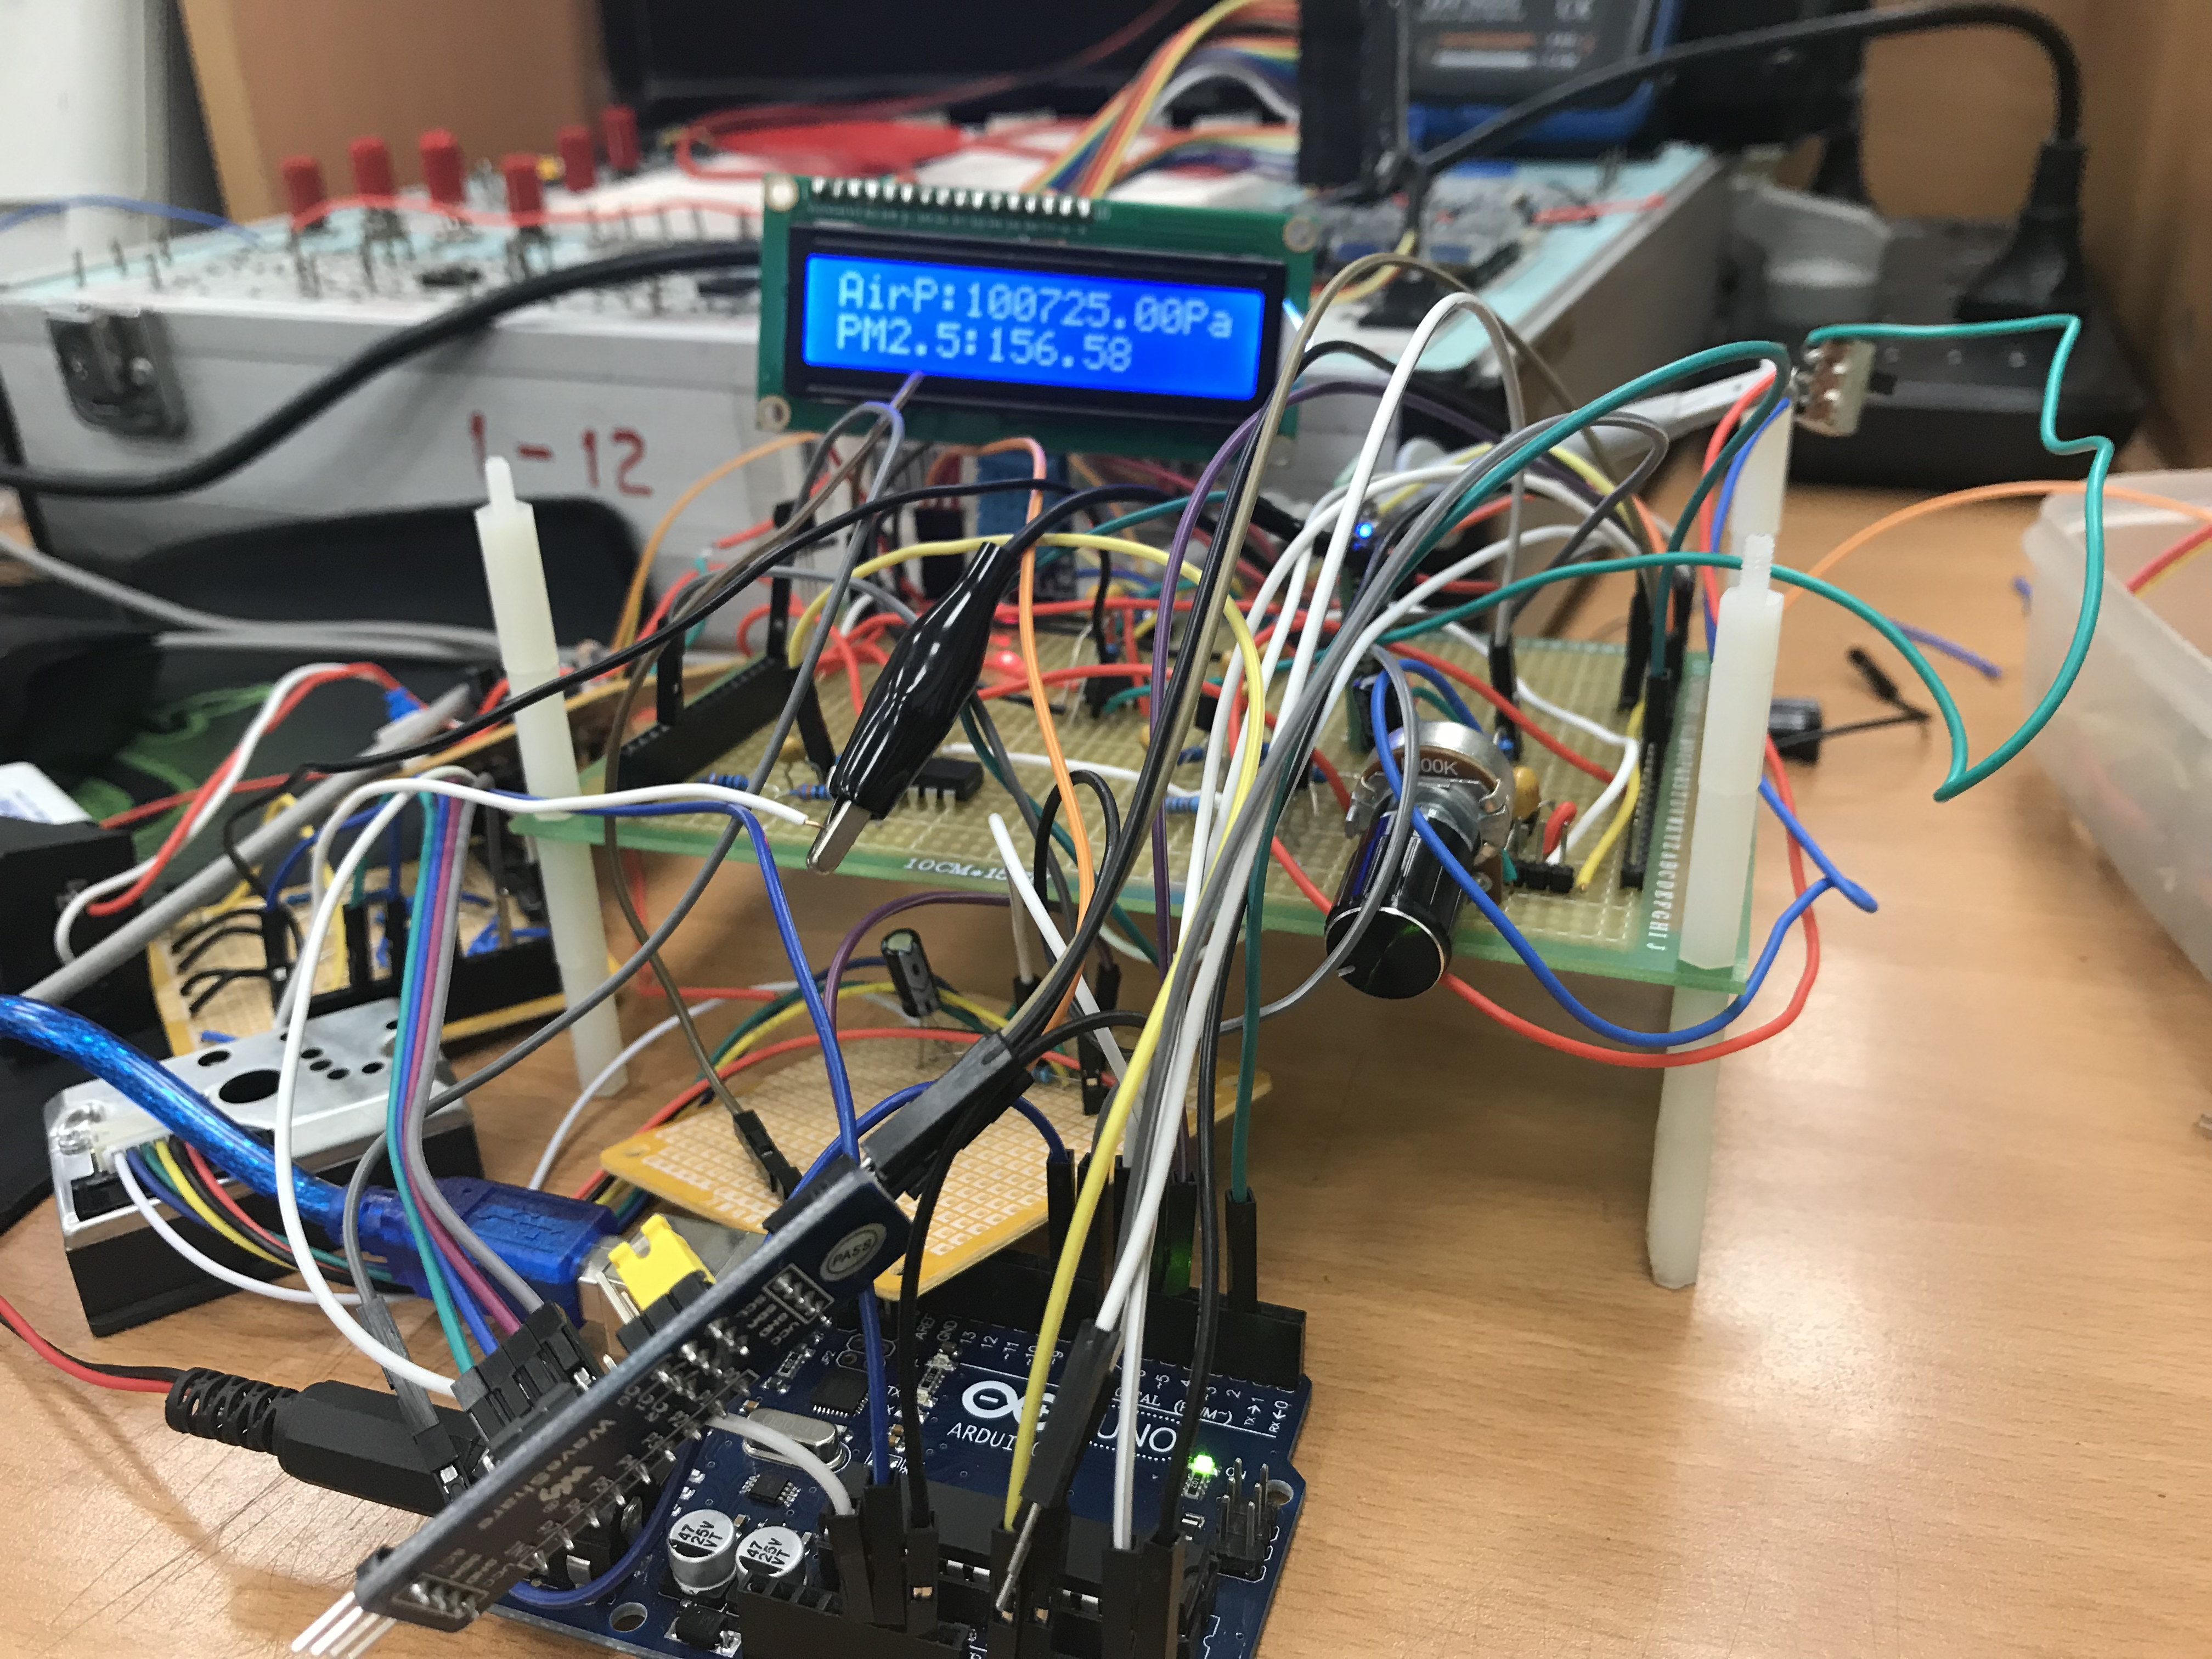
\includegraphics[width = 0.618\textwidth]{jiexian.jpg}
  \caption{实际接线图}
\end{figure}

\par{} 可以看出接线时十分复杂,极易将杜邦线错接或中途出现短接,这是由于我在焊接引出数据端时并不在板子的同一侧,以及引出VCC和GND过少,之后重新将DATA的引出规划在一侧,并且将VCC和GND和DATA在同一侧通过排针引出,便改善了这个问题。同时这个问题也提醒了我们在之后类似的设计中,例如万能板的焊接,走线采用统一的方式既能保证板子的整洁,也便于之后的调试。
\par{} \textbf{5.PCB制作问题}
\par{} 我们组曾在第一周尝试为电源管理模块制作PCB,而我们利用立创EDA制作了简单的PCB文件,如下图所示:
\begin{figure}[H]
  \centering
  \includegraphics[width = 0.618\textwidth]{PCB.png}
  \caption{PCB制作}
\end{figure}
\par{} 而之后在PCB制作完成后对自锁按键开关进行打孔的过程中,由于焊盘直径较小,将焊盘打没,则在焊接时锡直接流到了其他铜板上,无法有效的焊接自锁按键,最终PCB板作废。之后我们反思到首先是电源管理电路并不复杂,利用万能板会更方便一些,制作PCB耗时耗力,并且我们也吸取了经验,需要修改系统库中元件对于焊盘大小的设定,将焊盘设置够大以至于我们能够进行方便的打孔和焊接。

\par{} \textbf{6.Arduino板IO口资源紧张问题}
\par{} 由于我们的测量模块较多,需要与Arduino板直接相连的数据较多,因此显然的出现了IO口不够用的情况,这也是我们在设计时便考虑到的问题。而解决方法便是我们通过深入理解I2C协议,将机械键盘控制模块经过数字芯片PCF8574,让IO转I2C,使得气压模块,LCD显示模块和机械键盘模块均通过I2C协议传送数据,极大的节省了IO口的使用。

\subsection{软件问题分析}
\par{} 在软件层面,除了在利用控制字编写状态机出现的逻辑或语法上的小错误外,我们主要问题是动态内存和程序空间不足。Arduino UNO板在全局变量对动态内存使用超过75\%时便会报警,而内存的限制也限制了我们在功能和模块上的添加,因此我们也不得不相伴发节省动态内存和程序空间,至少能够达到我们的基本要求。

\par{} 而分析动态内存和程序存储空间不足的原因,可以从以下的三个方面得出:
\begin{itemize}
\item 部分类库冗余度高,占用了大量空间。
\item 主程序中的各分立的中间变量占用空间较多。
\item 打印数据前缀、单位等字符串常量也占用空间。
\end{itemize}

\par{} 因此对应于以上的三个方面,我们首先去精简类库,例如DHT11类库进行精简与修改(具体可见附录\ref{sec:all_src}-源代码\ref{src:dht11}79-82行等),其次我们换用BMP的官方库,去除了一些冗余的变量和函数,提高系统效率。

其次用更贴近底层和数字电路所学的知识进行系统的简化,节约内存。设计化简状态字,并$uint8\_t$类型存储,在状态判定转换时,依数电、计原所学,多用位操作以提升效率。(具体可见\ref{sec:digital_final},附录\ref{sec:all_src}-源代码\ref{src:EnvMeter}98-109行,224-252行等)

此外,用PROGMEM后缀和"F("string")"的宏,我们将提示字符常量和诸如GP2Y的采样时间常量等内容存入相对空间较大但读速度较慢且不能在工作时写入的flashrom中,能够有效的减少动态内存的占用,基于以上的设计和优化,我们最终在动态内存60\%的边缘完成了项目的设计。

\begin{figure}[H]
  \centering
  \includegraphics[width = 0.8\textwidth]{F_marco.jpg}
  \caption{资源使用优化举例——SD卡提示信息}
\end{figure}

\newpage
\bibliographystyle{plain}
\addcontentsline{toc}{section}{参考文献}
\bibliography{final_report.bib}

\newpage
\appendix


\section{完整源代码}
\label{sec:all_src}
整体项目可软件化的部分(包含数字系统程序、日志、文档、图片记录)我们均使用了github进行存储、迭代和同步,项目地址可见:\href{https://github.com/ZjGaothu/Electronic-design}{https://github.com/ZjGaothu/Electronic-design},以下给出最终版本的源代码

除此之外,我们还对dht11的通信协议进行了研究 \cite{dht11},是为优化dht11类库的通信和存储格式,达到节约动态内存使用的目的。项目原地址为\href{https://github.com/adidax/dht11}{https://github.com/adidax/dht11}

\lstinputlisting[caption = 数字主控源码-EnvMeter.ino, label = {src:EnvMeter}]{EnvMeter.ino}

以下为我们修改后的dht11库代码:

\lstinputlisting[caption = 修改后dht11库头文件-dht11.h]{dht11.h}

\lstinputlisting[caption = 修改后dht11库cpp文件-dht11.cpp, label = {src:dht11}]{dht11.cpp}

\lstinputlisting[caption = 数据分析使用的R代码]{recorder.R}

\newpage
\section{工作日志}
\label{sec:log}

除去手写的工作日志外,由于项目使用了git做文件管理,我们也一并将github统计的趋势给出,可视化我们的开发进度:

\begin{figure}[H]
  \centering
  \begin{minipage}[H]{0.48\textwidth}
    \begin{figure}[H]
      \centering
      \includegraphics[width = 0.8\textwidth]{git_contributor.jpg}
      \caption{github给出的时序可视化统计1}
    \end{figure}
  \end{minipage}
  \begin{minipage}[H]{0.48\textwidth}
    \begin{figure}[H]
      \centering
      \includegraphics[width = 0.8\textwidth]{git_frequency.jpg}
      \caption{github给出的时序可视化统计2}
    \end{figure}
  \end{minipage}
\end{figure}

以下是手写工作日志:

\begin{diary}{}{2019.07.01上午}

  电子设计小学期工作日的第一个上午,首先我们较为顺利地通过了预习验收,鼓舞了项目开始时的士气。
  
  此外,在等待验收的前前后后的过程中,我们主要使用\href{https://www.w3cschool.cn/arduino/}{W3Cschool的arduino教程},对我们所选的主控模块进行了简单的上手热身。主要了解了其整体的程序语法,控制流,IO功能和串口通信调试功能。
  
  接近上午调试结束时,我们还盘点了已有的一些模块。我们现有的模块有LCD显示屏,蓝牙通信模块,基本可以实现数字部分的功能。而模拟部分的模块,大部分传感器仍在配送,电源管理模块可先根据已有的备选芯片进行一定的调试。故而我们敲定了之后的计划,按照电源管理、arduino并行的方法进行调试。而LCD的调试相蓝牙模块调试调试而言比较简单,故先进行调试;并且另一路对电源管理模块调试的结束后,可以分人手去提前学习一下蓝牙模块的使用。得到近期调试优先度大纲如下:
  
  \begin{enumerate}
    \item arduino,LCD,串口联调;电源管理模块参数测试
    \item 蓝牙模块学习调试。
    \item 传感器模块的参数调试与联调。
    \item 其他基于分立元件(如光敏电阻)的外围传感电路设计
    \item 写数字系统整体代码框架
  \end{enumerate}
  
  \end{diary}
  
  \begin{diary}{}{2019.07.01下午}
  
  \par{}在经过上午的验收以及上手热身后,我们在下午正式开启了设计与调试,由于大多数传感器还没有送达,我们手中已有的模块是arduino uno主控模块和LCD1602液晶显示模块,为了减少IO的使用,我们特地前往中发电子大厦购买了I2C转接板,将16引脚方便的减少为4引脚和arduino相连接。
  
  在购置回转接板后,我们一方面开始学习LCD1602与arduino的硬件连接方法,以及其各个引脚的说明,并且在利用已有的LiquidCrystal库函数的情况下,尝试进行了字符数据的显示,成果如下:
  \begin{figure}[H]
    \centering
    \includegraphics[width = 0.53\textwidth]{chuan2.jpg}
    \caption{LCD字符显示}
  \end{figure}
  起初并不能显示,后来我们很快发现是转接板电位器的问题,转接板电位器直接控制了LCD显示的亮度,因此在使用镊子改变电位到合适的亮度后便能观察到字符。在能够显示字符后,我们进一步结合上午的学习进行了串口LCD通信联调,使得在键盘上实时输入字符在LCD上进行显示,这是我们之后显示模块的重要基础,我们拍摄成果的照片如下:
  \begin{figure}[H]
    \centering
    \includegraphics[width = 0.53\textwidth]{chuan1.jpg}
    \caption{LCD串口通信联调}
  \end{figure}
  另一方面,我们组在调试LCD的同时,对电源管理电路进行了实际的检测,我们计划使用9V的干电池,而恰好在实验室中找到一块电源管理的模块,能够在小于12V输入的情况下,输出5V/3.3V的直流电压,我们类比于电网$10\%$的波动,使用$8V\sim 10V$的50Hz正弦波作为输出,观察两输出的电压情况,结果十分令人满意,根据示波器的显示,以及自动测量的结果,能够得到纹波非常小的直流电压,并十分接近其标称的输出,记录如下图所示:
  \begin{figure}[H]
    \begin{minipage}[t]{0.45\linewidth}
        \centering
        \includegraphics[width=6cm]{dy1.png}
        \caption{3.3V稳压输出}
    \end{minipage}%
        \hfill
    \begin{minipage}[t]{0.45\linewidth}
        \centering
        \includegraphics[width=6cm]{dy2.png}
        \caption{5V稳压输出}
    \end{minipage}
  \end{figure}
  其中黄色线为稳压输出,绿色线为输入,验证了该电源管理模块能够提供理想的供电电压,在TI公司的样片到来之前为我们的电源管理提供了替代。
  
  在下午收工以后我们另外找到一片蓝牙模块,计划于明天开启蓝牙模块的调试以及DHT11的湿度模块的调试,并通过LiquidCrystal库编写代码,实现自己需要的函数的头文件。
  
  \end{diary}
  
  \begin{diary}{2019.07.02上午}{DHT11温湿模块与蓝牙模块调试}
  \par{}电子设计小学期工作日的第二个上午,我们明显加快了调试的进度,在昨天初步调试LCD1602后,今天我们进一步同时开始调试蓝牙模块和DHT11温湿模块。
  
  首先,上午蓝牙模块的调试并不是十分顺利,中间遇到了一些连接的问题,进度稍慢,而温度湿度传感器模块借助于Arduino官网可查找的dht11的库,可以很快的进行实现。我们设置没两秒更新并发送一次数据,可以在串口接受到数据。之后便很方便地将数据
  
  为了验证其正确性,我们将传感器分别在室内与室外进行了测量,结果表明室外比室内温度大约高$3^\circ C$左右,湿度也稍高于室内,符合实际情况,测量结果如下图\ref{img1}记录:
  \begin{figure}[H]
    \centering
    \includegraphics[width = 0.53\textwidth]{temp1.jpg}
    \caption{温度湿度测量与LCD显示}
    \label{img1}
  \end{figure}
  
  该LCD显示了当前教室的室温和室内湿度。
  整体上温度湿度模块由于能够直接输出校准后的数字信号,所以调试过程比较顺利,只是在单位的输出时$^{\circ}C$的符号难以直接输出,库中的print()函数无法输出该字符,需要去自定义字符,否则会输出响应的日文,因此我最终采用了print((char)233)在其中一格的$5\times 7$矩阵先输出“度”的上标,再输出C来完成单位的显示。
  
  此外,我们修改了$LiquidCrystal\_I2C$库的内容,将其精简并增加了和串口联调的功能,成为我们可以使用的$serial\_lcd$库,其中的函数实现原理大致与官方库相同。此后该模块恰好能够利用该屏幕进行显示,因此我们考虑了一下多模块测量的显示方法,我们选用TTP226电容触摸开关进行显示内容的选择,不同的开关控制不同内容的显示,因此我们目前手头只有TTP224,并用其进行测试其触摸效果,结果十分令人满意。
  
  而另一模块,蓝牙模块的调试,能够初步和设备进行连接,但基于Arduino进行数据通讯仍具有一定的问题,有待下午进一步调试。
  
  \end{diary}
  
  
  \begin{diary}{2019.07.02下午}{蓝牙模块调试和系统架构细节讨论}
  
  在下午我们完成了蓝牙模块的调试,经过排查,发现是使用的蓝牙模块已经进行了配置,和出厂设置不同,厂方给出的设置方案不能直接使用。在简单了解AT指令集后,我们迂回使用USB转TTL的芯片,先对蓝牙模块进行恢复出厂设置,便可按照厂方文档进行调试。按照应用情景,我们将蓝牙模块设置为从机,波特率设置为9600(之后可能会调节到更低以节省功耗),简单测试了手机通过蓝牙模块、电脑通过蓝牙模块与arduino的通信,顺利完成数据的收发并能做出简单的响应,可以预料到能与后续的模块完成连接。
  
  此外,气压传感器BMP180的特性测试和简单实用调试也在今天下午完成。此外在考虑微波雷达探测人体存在的实际情况,我们认为可能需要做一定的角度的扫描检测,故而在实验末尾简单阅读了舵机的工作原理和操作例程,这是一个控制模块,可以预料到调试环节不一定顺利。但是这是一个数字驱动的模块,可以在今晚先将大部分功能点实现,其他的预想功能如根据雷达信号的反旋转舵机,需要之后联调实现。
  
  最后,已经看到的情况是,由于外设较多,arduino的IO资源已经有些紧张,而且各外设的使用方式不一,有直接用IO功能进行读写,有用I2C进行通信。我们敲定方案是用IO转I2C和I2C扩展板,实现一个统一的数据总线结构,方便整体系统调试。另外我们还需要一个数据存储媒介给仪器记录实验数据。所以在今天下午实验结束后,我们还去中关村中发市场进行了相关器件的采购。
  
  \end{diary}
  
  
  \begin{diary}{2019.07.03上午}{舵机、SD卡、LCD12864、红外收发调试}
    
  电子设计小学期工作日的第三个上午,我们继续对已有的模块进行测试。我们在昨天的采购时重新购置了一块较大的液晶显示屏,型号为LCD12864,是一块分辨率为128*64的显示屏,并带有中文字库,相比与1602具有更大的优势,首先我们先去将其20引脚焊好排针,之后我们利用了已有的一个简单库函数,并且对其进行函数的补充与丰富,例如清除光标等函数,并对其进行了显示的测试,测试结果能够清楚的显示如下图\ref{img2},但是发现该屏幕对电磁干扰非常敏感,在硬件接线有扰动或者其他电磁干扰的情况下,会出现乱码的情况,这是我们进一步需要解决的问题。
  \begin{figure}[H]
    \centering
    \includegraphics[width = 0.53\textwidth]{12864.jpg}
    \caption{12864显示}
    \label{img2}
  \end{figure}
  
  除此之外,我们调试使得舵机能够正常运转,我们希望借助180$^{\circ}$旋转的舵机能够帮助微波雷达模块对室内的人体进行感应与检测,扩大其检测范围。在调通舵机后,我们开始了对SD卡存储的调试,初步能够实现通过Arduino将数据发送的SD卡进行存储。并且在舵机模块和SD卡模块的类库的使用中,我们注意到从类库生成的对象较大(一个舵机大约占用动态内存的20\%、一个SD文件对象大约占用动态内存的50\%),故而我们讨论了两种解决方案,第一是精简类库,减少内存消耗,二是使用PROGMEM后缀,将变量存储在flashrom中。第二个解决方案用于对读写实时性的要求不高的场景,初步确认SD卡文件对象内存占用大的问题可以使用这个方式得以解决。这是因为将测量数据转存到SD卡的操作本身就是外存文件操作,速度较低。而舵机对象的问题推迟到最后联调时视情况解决。此外我们还进行了红外收发模块的调试和标定:得到编码如下:
  
  \begin{figure}[H]
    \centering
    \includegraphics[width = 0.2\textwidth]{controller_code.png}
    \caption{红外遥控编码}
  \end{figure}
  
  并且我们进一步讨论总线的管理方法,由于IO资源较少,而待测量变化频率一般较低,我们希望能够在每次轮询周期内利用一根总线分别选通各传感器进行数据传输,因此我们需要搭建数据选择电路,为此我们在午饭时再次前往中发市场购置数据选择器等器件。
  
  \end{diary}
  
  \begin{diary}{2019.07.03下午}{元件增购与总线结构讨论}
    
    根据课上所学的知识,我们在中发市场增购了八输入数据选择器74151,用做输入总线的设计。此外采购了GPIO转I2C的芯片PCF8574。I2C在LCD1602调试时我们接触到的一个串行通信协议。在下午的正是调试中,我们两路并行进行,一方面对购得的元件进行逻辑测试,另一方面学习理解I2C协议。以下是在PCF8574的数据手册中截图得到的关于I2C的介绍。大约分为主机发送起止命令、选择地址和读写模式,以及从机被读或被写时按8位数据位一位应答位的串行数据传输形式。
  
  \begin{figure}[H]
    \centering
    \includegraphics[width = 0.8\textwidth]{I2C.png}
    \caption{I2C数据传输举例(从数据手册中摘录)}
  \end{figure}
  
  在简单讨论后,我们决定先试用I2C进行总线管理。主要出于以下几个目的:
  
  \begin{enumerate}
    \item I2C适用于通信速率低的情景,在轮询传感器时,符合这个特点。
    \item I2C是相对主流的通信协议,可以方便后续拓展。
    \item I2C协议读写均支持,是更完整意义上的总线形式,比起我们用数据选择器设计的只读总线结构更为合理,也可以把读传感器值和内容显示等读写操作统一在一个时序中,让程序更为统一。
    \item I2C协议要求我们对时序电路有更好的理解,我们也想在这方面挑战一下自己。
  \end{enumerate}
  
  \end{diary}
  
  
  \begin{diary}{2019.07.04上午}{I2C总线协议理解与讨论}
  
  在网购元件到来前的最后一个上午,我们首先进一步研究I2C总线协议,为我们之后的总线架构做出准备与铺垫。我们阅读并参透了LiquidCrystal的库函数,进一步参透了解I2C传输协议。
  
  除此之外,我们另一路开始为下午的模块调试进行准备,计划在下午能够完成所有模块的调试使得明天可以进行各模块的联调。首先查阅了GP2Y1050AU0F的模拟输出特性,以此为基础先编写好程序,并进一步连接其接线,由于我们已知其为模拟输出,自然考虑到传感器的输出会受到噪声的影响,为了改进输出特性,我们提前设计好了VCVS低通滤波电路,滤波特性如下:
  \begin{figure}[H]
    \centering
    \includegraphics[width = 0.75\textwidth]{bote.png}
    \caption{低通滤波特性}
  \end{figure}
  
  可见我们已经能够实现低通滤波的仿真,使得该模块的模拟输出稳定,并且在之后综合比较了LCD1602和LCD12864的显示效果以及调试难度,由于12864的显示常常因电磁干扰而显示乱码,我们仍决定采用1602。在上午的工作接近末尾时,我们大概完整的阅读并理解完I2C协议与LCD显示的库函数,我们在网上购置的模块也终于到来,为我们开发工作的进度有进一步推动。
  
  \end{diary}
  
  \begin{diary}{2019.07.04下午}{PM2.5传感器、微波雷达、光强测量电路的调试}
    
  下午模块一到,我们便首先对PM2.5检测的GP2Y1050AU0F传感器的特性进行标定。室内空气质量好,故传感器的模拟输出较低,且用示波器看不到明显变化。在回忆了传感器的原理,是通过对管对自己发射的光信号进行放大,而收集槽中的灰尘会部分挡光导致输出示数变化。故而我们简单用铅笔伸入收集槽的方法对传感器特性进行测试。下图为伸入铅笔后的,滤波前和滤波后的输出:
  
  \begin{figure}[H]
    \begin{minipage}[H]{0.48\textwidth}
      \begin{figure}[H]
        \centering
        \includegraphics[width = 0.8\textwidth]{before_fliter.png}
        \caption{灰尘传感器滤波前输出}
      \end{figure}
    \end{minipage}
    \begin{minipage}[H]{0.48\textwidth}
      \begin{figure}[H]
        \centering
        \includegraphics[width = 0.8\textwidth]{after_fliter.png}
        \caption{灰尘传感器滤波后输出}
      \end{figure}
    \end{minipage}
  \end{figure}
  
  可以看到,滤波后输出质量明显提高。并且可以想到的是,在本次实验中的噪声主要来自铅笔的晃动,而实际测量中的噪声可能来自空气颗粒的随机运动,应该会是更大的噪声,故而进行这次滤波是很有必要的。
  
  微波雷达的生物探测功能已经进行了验证,在所需范围内有生物移动时会得到高电平输出,并且其穿透探测的功能也得到了验证。但是由于小组中一人的工作台的示波器工作异常,故没有记录详细波形。
  
  最后是光强测量电路的设计、仿真和调试。手边拥有的光敏元件是光敏电阻,在查阅了光敏电阻的光敏特性曲线,其理想的关系应当是
  
  \begin{equation*}
    \ln(\frac{R}{R_0}) \propto \ln(\frac{I}{I_0})
  \end{equation*}
  
  最直接的想法是用分压关系将反映成电阻变化的光强变化作为电压信号,接入后级的放大和滤波电路后得到检测信号。但分压网络的缺点是会在分子和分母都出现变化的电阻,故而电压信号和待测物理量不是线性关系,需要后级的数字系统用计算处理。而在本例中,问题更为复杂了,因为待测物理量和电阻值的变化并非线性关系,导致了一个超越方程,难以求解。若使用计算机上常用的方式,即基于试根的方法会比较占用MCU本就不多的计算资源,很得不偿失。故而转换思路,使用555压控振荡器做电阻-频率转换。首先进行仿真验证,搭接如下电路。
  
  \begin{figure}[H]
    \centering
    \includegraphics[width = 0.618\textwidth]{555_sim.jpg}
    \caption{基于555多谐振荡电路的光强检测计}
  \end{figure}
  
  图中标注LDR的即为光敏电阻,左侧方案更为简洁,并且得到的是占空比$50\%$的方波,更好进行检测。进行优先的仿真和调试。简单的数学推导后得到输出波形振荡周期$T$与光敏电阻值$R$成正比,是一个简单的关系。故而可以避免解超越方程的尴尬。仿真振荡波形如下,但由于实际电路需要对光强进行标定,实际测量的调试在明天携带进行,仿真波形仅用于确认电路可正常工作。此外,基于555的测量电路还有在光敏电阻上电压值较为恒定,输出电平标准稳定不容易损害后级电路和低功耗的特点,是我们认为较之于基于分压电路的设计方案更好更简洁的解决方案。
  
  \begin{figure}[H]
    \centering
    \includegraphics[width = 0.618\textwidth]{555_sim_osc.jpg}
    \caption{555多谐振荡光强测量电阻仿真波形图}
  \end{figure}
  
  \end{diary}
  \begin{diary}{2019.07.05上午}{模块联调初步搭建与电源管理模块PCB设计}
  
    \par{}在工作日的第五个上午我们在调试通过各种模块串口数据收发的基础上,开始了所有模块的联合调试,此外,我们在昨晚收到了TI公司的样片,电源管理模块使用的芯片TPSM84,也进一步对电源管理模块进行测试。
  
    首先在面包板上搭建电源管理模块的电路,输入$8\sim 10$V的正弦波,观察稳定输出的结果,如下图所示:
  
  \begin{figure}[H]
    \centering
    \includegraphics[width = 0.618\textwidth]{dianyuan.png}
    \caption{电源管理模块}
  \end{figure}
  
  在输入正弦波存在毛刺的情况下,输出电压非常稳定,波动在毫伏级别,因此我们也验证了该模块能够正常工作,因此,我们计划将电源管理模块单独设计出一块PCB板进行系统的供电,由于本身的电源管理模块部分比较简单,因此也便于我们去添加额外的开关和电源指示灯,我们在上午绘制好了电源管理模块的PCB图并送去制版,如下图所示:
  \begin{figure}[H]
    \centering
    \includegraphics[width = 0.58\textwidth]{pcb.png}
    \caption{电源管理模块PCB绘制}
  \end{figure}
  在PCB绘制的过程中,由于我们无法从元件库找到TPSM84芯片,因此查阅其datasheet换算单位后自己制作出了TPSM84的PCB模块,并且后来由于添加开关我们现找了自锁的按动开关,查阅其引脚和内部连接后进行接线,初次绘制PCB耗费了一定的时间。
  
  另一路工作首先对基于555的光强检测电路进行了简单的实物搭接和收尾验证,得到波形如下:
  
  \begin{figure}[H]
    \begin{minipage}[H]{0.48\textwidth}
      \begin{figure}[H]
        \centering
        \includegraphics[width = 0.8\textwidth]{light_osc.png}
        \caption{光强检测电路波形(室内正常环境)}
      \end{figure}
    \end{minipage}
    \begin{minipage}[H]{0.48\textwidth}
      \begin{figure}[H]
        \centering
        \includegraphics[width = 0.8\textwidth]{dark_osc.png}
        \caption{光强检测电路波形(遮挡光敏电阻)}
      \end{figure}
    \end{minipage}
  \end{figure}
  
  可以从波形可以定性看到,由于光强减弱,光敏电阻阻值的增加,振荡周期增加,频率减小,符合定性规律。另外一方面,参考室内$300\text{lx}$,而遮挡时,近似看为野外室外环境光强$1lx$扣除偏移量,验证其对数值的近似线性关系。
  
  之后的工作计划于面包板上先实现硬件的连接,随着硬件的搭建我们同时开始软件方面的引脚分配,初步在无总线的情况下在Arduino串口轮询读取数据,若其能够联合正常工作并读取数据,则可进一步设计PCB和添加总线方案。我们已经在面包板上完成了基于555的光强检测计,DHT温度湿度模块,BMP180气压检测和PM2.5模块的低通滤波部分,以及红外遥控模块,如下图所示:
  \begin{figure}[H]
    \centering
    \includegraphics[width = 0.58\textwidth]{lianhe.jpg}
    \caption{联合调试部分硬件}
  \end{figure}
  在下午的工作中我们将进一步进行搭建以及编写ino进行串口数据读取,如果PCB制作完成则会进一步焊接与测试。
  
  
  \end{diary}
  
  \begin{diary}{2019.07.05下午}{模块联调}
  
  下午实验开始后,我们打印的PCB很快就做好了,所以我们兵分两路,一路进行PCB的焊接,一路继续进行联调电路的搭接。最后的搭接完成后,我们在面包板上放置了基于555的光强检测计,DHT温度湿度模块,BMP180气压检测和PM2.5模块和其配套的低通滤波器,红外接收管、微波雷达和按键和其对应总线管理的数字模块。如下图(图片为实验结束后拍摄,当时为了携带方便,体积较大的PM2.5传感器和疑似烧坏的按键没有连接)
  
  \begin{figure}[H]
    \centering
    \includegraphics[width = 0.618\textwidth]{all_outside_circuit.jpg}
    \caption{外围电路联调}
  \end{figure}
  
  另一路在进行PCB板焊接时,由于按钮插孔的焊盘过小,我们失手将其焊落,难以进行修补。这给了我们一定的教训,PCB印制结束后,并不意味着工序的结束,在实验的任何一个阶段都要小心操作。为了保证进度,达成本周实验结束后将外围硬件部分联调通过,方便周末写软件部分的目的,我们选择换用万能板做电源管理模块,迅速搭接如下电路,并将电源管理模块加入联调。
  
  \begin{figure}[H]
    \centering
    \includegraphics[width = 0.618\textwidth]{V_src.jpg}
    \caption{电源管理模块实物}
  \end{figure}
  
  最后在用示波器简单验证各模块输出,再辅助简单的串口打印检测量的程序,我们验证了外围电路联调的基本通过,给周末进行软件部分调试打好了坚实的基础。
  \end{diary}
  
  
  \begin{diary}{2019.07.06上午}{联合检测代码与元件采购}
  \par{}在经过周五的电源的准备,为我们的联合调试提供了基础,我们进一步推动了工作的进度,开始想办法在节省动态内存的情况下编写代码,首先我们在检测部分进行联合调试,我们结合了温度湿度气压与灰尘和基于555的光强检测在串口显示数据。
  
  而在上午的调试过程中我们遇到了DHT11模块显示不准的问题,我们在测试的过程中发现了串口显示的温度要明显的高于室温5$^{\circ}C$左右的,并且会在checksum的时候报告checksum error,据查阅是串口数据传输的校验位错误,而我们在仔细研究了dht11.h的库后发现旧版本的dht库函数在检验sum和中将小数部分当做零处理,而我们现在使用的传感器小数部分并不等于0,将其进行如下所示的修改便可:
  \begin{figure}[H]
    \centering
    \includegraphics[width = 0.618\textwidth]{code.png}
    \caption{库函数修改}
  \end{figure}
  
  在修改后明显测量数据在正常的室温范围内,并且相较于起初的单元模块调试,能够精确的小数点后两位,有较大的精度上的改善,除此之外,我们前往中发市场采购了中型的洞洞板,为检测模块的固定进行了进一步的准备。
  
  \end{diary}
  
  
  \begin{diary}{2019.07.06下午}{通信部分代码编写与焊接设计}
  \par{} 在所有的检测模块都能够正常工作后,我们一路进行代码的完善补充另一路进行焊接的设置,首先是代码层面,开始了将蓝牙部分以及舵机和雷达部分接口的设计,并将蓝牙与SD card部分的库与代码加入我们总的debug代码中,进行了编译以及调试,效果良好,并且,我们为了节省内存,查阅了一些arduino编程的技巧以及变量运用的技巧,尽量减少内存的占用。
  
  而另一路则将面包板的检测部分,设计在洞洞板上进行焊接,由于在周五的焊接中发现洞洞板在接线方面不太方便,因此首先查阅了洞洞板焊接的技巧,其中接线主要分为两种方法,其中一种为连焊走锡式焊法,通过焊锡来使电气连接,另一种方法为背面飞线式,通过导线在洞洞板背面实现电气连接,由于走锡式焊法极易造成错误,难以修改,因此我们决定采用飞线式焊法,并且做了以下简单的设计:
  
  \begin{figure}[H]
    \centering
    \includegraphics[width = 0.618\textwidth]{han.jpg}
    \caption{焊接简单设计}
  \end{figure}
  我们此板打算只焊接检测部分,并且电源管理部分单独用一块小板,显示部分另用一块板进行共地处理。
  
  \end{diary}
  
  \begin{diary}{2019.07.07上午}{显示方法设计讨论与代码完善}
  
  在电子设计小学期第六天的上午,我们在其他模块的代码完成后,开始了显示部分的讨论,首先是硬件上对显示的控制,我们列举了需要显示的内容:温度,湿度,气压,灰尘,雷达监测、光强这六项内容,初步设计通过四个独立按键来控制,由于LCD1602仅为16*2的显示,因此每一个测量指标需要占用一行,我们采用翻页设置,分别利用两个按键进行上翻和下翻,另一个按键为滚屏的开始/停止键,滚动屏幕每次滚动一行,另一按键为灵敏度调节,开启此按键后,通过另一电位器调节检测周期,我们设计基准的周期为1s。而另一方面利用红外遥控进行同样的控制,另外单独通过按键来改变显示的顺序,同样通过蓝牙进行串口的数据传输,类似于电脑的串口监视器。这是我们对于显示部分的讨论结果。
  
  在讨论结果设计好后,便开始将显示部分加入我们的主代码,具体使用的函数见于报告附的代码中,基本的实现方法和我们模块调试大同小异,只是在翻页设置我们添加了状态与按键编码的练习,通过逻辑运算来切换状态,至此我们已经完成了整体的所有部分的代码,动态内存也达到了$73\%$,即将到的$75\%$的阈值。只需在周一进行代码的测试。
  
  \end{diary}
  
  
  
  \begin{diary}{2019.07.07下午}{混沌电路的设计以及独立按键硬件设计}
  
  在完成了整体代码的设计后,我们便需要在硬件部分进行设计,也即我们设计的独立按键的四个功能:滚屏、上下翻页和灵敏度调节。我们所需要的是在按下时得到其高电平,因此我们可以通过对四个键进行编码,经过IO转I2C接口后直接以I2C形式给到Arduino的SDA和SCL,在内部对其进行地址分配即可,我们通过四个独立按键给出的编码来进行状态的切换,而设计以简单为原则,参照FPGA独立按键的原理,采用上拉电阻和下拉电阻便可简单的解决问题。
  \begin{figure}[H]
    \centering
    \includegraphics[width = 0.48\textwidth]{dianping.png}
    \caption{独立按键设计}
  \end{figure}
  
  这部分设计比较简单,因此还需明天在实验室进行显示、通信、检测三大部分的联合调试,再具体的发现问题。
  
  除此之外,由于雷达需要进行旋转扫描,而针对于室内情况,随机角度的扫描更符合对环境检测的需求,而不是定时的进行旋转,因此舵机旋转角度的设置便可有产生随机数来进行确定,我们初步的思路为产生电压值随机的模拟电压,通过Arduino的模拟接口来读入模拟电压在程序内部进行进一步的随机角度设置。
  
  但设计的关键之处在于随机电压的产生,我们在查找文献后找到了一种混沌电路的发生方法,其原理为使用RC振荡电路但使其震荡点不稳定从而使振荡频率非周期变化,来产生混沌。其原理电路如下:
  \begin{figure}[H]
    \centering
    \includegraphics[width = 0.58\textwidth]{hundun.png}
    \caption{混沌电路}
  \end{figure}
  
  在修改其参数便于实验室中找到已有元件后,得到稍规律化后的混沌电路,但观察其相图仍为混沌状态,仿真结果如下:
  \begin{figure}[H]
    \centering
    \includegraphics[width = 0.58\textwidth]{hundun1.png}
    \caption{混沌电路仿真}
  \end{figure}
  
  我们进一步在面包板上搭建了混沌电路,计划周一上工后利用电位器进行调节到混沌状态,至此我们周末的调试基本结束,总体的代码也已基本完成,若在周一所有模块联调后正常工作,我们便进行焊接与外围电路位置分配的设计。
  \end{diary}
  
  
  \begin{diary}{2019.07.08上午}{联调验证与焊接}
  
  得益于周末的顺利工作,我们上午先在面包板上再次进行验证性的联调,联调通过的模块进行焊接,其他模块继续调试。按照两路并行的模式继续工作。调试时,大部分的检测模块都顺利工作,但是GP2Y灰尘传感器工作不正常。
  
  通过对程序不断注释与控制变量,我们逐次发现了一下几个原因:
  \begin{itemize}
    \item arduino与SD卡通信时需要用到SPI总线协议,故除SD卡选通端,其他端口在库中已经写好。而这写好的引脚中的一个与GP2Y传感器使用的LED的IO口发生冲突,导致无法驱动传感器内部的LED进行闪烁,进而检测到的模拟量始终为0,修改了这个错误后,我们直接使用模拟口读入数据在正常范围内。
    \item 滤波后输出过低。使用示波器观察比照低通滤波前后的波形发现我们之前的滤波手段并不正确。为保护红外管,GP2Y1050数据手册建议的是需要采样时,按照给LED一个脉冲,在脉冲末端读取模拟输出,且建议的检测LED闪烁时长不得少于$10ms$,采样点在LED启动后$280ms$之后。而之前的截止频率在过低,导致低通滤波直接将检测信号的很多有效分量滤除,自然无法检测到模拟量,因此我们修改了参数的设置,将截止频率设置在$3kHz$以上。此外,还发现了之前的通带放大倍数为2,在传感器模拟端口输出较大,大于$2.5V$时,2倍的通带放大倍数可能导致输出信号大于$5V$,会在检测浓度较高时超出1023的量程,并且有可能损坏主控板模拟输入口。因此,我们将通带放大倍数修改为1,也即滤波器通带等效为电压跟随器,对应修改其他电阻,保证NP间的直流通路下,对地电阻相同,保证直流对称即可。
  \end{itemize}
  
  
  \end{diary}
  
  
  
  \begin{diary}{2019.07.08下午}{遥控测试、混沌电路调试与万能板焊接}
  \par{}
  
  
  下午继续兵分两路的工作,一路进行模块测试,一路进行模块焊接,将测试通过的模块逐个焊接到万能板上。首先是调试的部分,在红外遥控控制的调试中遇到了一些小问题,例如state的变化并非和按下的按键相匹配,经查找后发现是代码中逻辑运算优先级的问题:
  \begin{figure}[H]
    \centering
    \includegraphics[width = 0.618\textwidth]{code1.png}
    \caption{红外遥控编码}
  \end{figure}
  如上图所示由于运算优先运算后面的等于号,再运算按位与,和我们的初衷相反,因此我们手动修改运算优先级后解决了问题,并且通过和LCD显示的联调可以通过遥控实现上下翻页和滚屏的开始与停止操作,因此红外模块也可以交去焊接。
  
  在红外调试之后,开始了另一部分模拟电路的调试,也即昨天所设计舵机转动的混沌电路,而我们在调试的过程中始终无法使其产生平衡点不稳定的振荡,总是出现一定的周期化,我们检查了三极管的连接,使用参数的阻值,不断修改电位器,不断重新仿真,始终没有得到混沌的输出。
  
  
  而焊接部分则是比较消耗时间的部分,由于焊接人数众多,因此不得不有很多的等待时间,不过我们对于模块的焊接短短续续持续了一整天,并且想要通过排针来引出data端,既方便又美观。至此,我们已经焊接完成的模块是DHT11检测部分,PM2.5检测部分,红外遥控部分,基于555的光强检测部分,PM2.5VCVS低通滤波检测,舵机部分,电源管理电路部分,如下图所示:
  \begin{figure}[H]
    \centering
    \includegraphics[width = 0.618\textwidth]{hanjie.jpg}
    \caption{焊接成果}
  \end{figure}
  
  临近5点,我们还有部分,待收尾的工作有:混沌电路的调试和部分连接点的焊接。我们决定在晚上解决这些问题,保证进度,方便明天的调试。
  
  \end{diary}
  
  \begin{diary}{2019.07.09上午}{焊接与中断源}
  
  在昨晚的焊接之后,我们将模块基本固化到了万能板上面,在早上进行简单的联调后,发现除了带动雷达的舵机不转和灰尘传感器的滤波输出不正常之外,其他模块工作正常,与数字系统联调能正常工作。于是我们开始进行这些问题模块的排查。另一方面,我们注意到我们设计的系统需要的采样频率不高,而使用数字系统本身的延时函数进行轮询的周期的调节,一方面程序复杂,另一方面延时时,单片机仍然工作在正常状态,功耗较大。
  
  在简单讨论后,我们决定设计一个长周期的方波发生器,作为中断输入,而单片机调用下级传感器的做采样的函数,即作为中断服务程序,这样在非采样时,数字系统可以工作在睡眠状态,有效降低功耗,也可以解决LCD在更新时的闪烁问题。从这里,我们进一步为系统增加了一个功能,即自动采样和手动采样,用一个开关切换方波输出和另一个555单稳态电路输出,后者作为即可作为手动采样的触发信号,这样可以帮助使用者标定房间内不同地方的相关参数。
    
  \end{diary}
  
  \begin{diary}{2019.07.09下午}{焊接与排错}
  
  上午舵机不工作和滤波器输出异常的错误,经过仔细的排查,发现是这两个元件的地端未接好,用示波器显示为约$5V$,再经过排查,发现是地线那部分出现了虚焊,与电源管理模块共同作用,导致了一定的浮动电压,进而导致运放输出基准变为$5V$,故而滤波后输出总是出现超过测量范围的异常。而舵机两端相当于没有供电,也因此不转。在搞清楚问题后,我们对那一部分重新焊接,排除了错误。
  
  此外,下午的焊接也有很大收获,我们基本完成了焊接,决定晚上进行收尾联调和包装盒的制作。
      
  \end{diary}
  
  \begin{diary}{2019.07.10上午}{首次验收和第二次验收}
    
  上午一到,进行简单的联调复现,我们进行了首次验收,主要实现的功能有:
  
  \begin{itemize}
    \item 5个物理量的测量,包括温度、湿度、气压、光强和PM2.5颗粒物浓度。
    \item 做一定的有效换算,如把气压转换为标准大气压、光强用为科学计数法、PM2.5浓度到空气质量指数的换算并且显示。
    \item 实现了一定的状态切换与显示,可以让LCD进行滚动显示和手动翻页的切换。
  \end{itemize}
  
  在第一次验收通过后,极大的增强了我们的信心,按照预计方案,我们将各数值的采样作为一个采样用的总函数题,用两路切换的,加入滑动变阻器的555多谐振荡电路、555单稳态电路,作为可调时长的自动采样和手动采样功能,进行调试。这样中断触发的形式,还能让arduino进入睡眠模式,让整体系统功耗更低,使用时间更长。完成了增加的功能,并且由此进行了第二次验收。助教也认为认为自动手动采样的功能比较符合我们设计的测量仪器的功能要求,并且建议我们在装箱后,给伸出的用于调节采样市场的滑动变阻器周围进行时长定标,让仪器使用更人性化。
  
  \end{diary}
  
  \begin{diary}{2019.07.10下午}{电路故障排查与存储功能、蓝牙通信、上位机通信验收}
  
  在经过上午的验收后,我们的电池很快没电,在充电后再次上电发现出现了我们长遇到的问题,DHT11的LED在未通电时便亮了,这直接告诉我们出现了共地错误,而我们不加电池模块时,便没有出现这个问题,我们将问题聚焦在电池模块,经过万用表各个共地点排查,发现了电池的地和Arduino的地之间有2.4V左右的电压,而我们经过测量,发现Arduino地线良好,而电池连接线地线也同样是电气短接的,这着实让人困惑,我们这时已经怀疑是电池座的问题,无奈先剪短了已经焊接的和电源管理部分的连接,开始单独排查电源和Arduino,现象非常显然,电池无法通过供电口驱动Arduino,且此时电池已经充满电,在找助教寻求帮助后确认是电池盒地线内部可能发现断接或连接不牢,换了电池盒立刻解决了问题,也让已经验收过的我们对此类问题更加警觉与重视。
  
  在恢复了功能后,我们开始调试SD卡存储功能,通过将数据以csv的格式存储在sd card上,我们以电位器调节到10s的采样周期,读取了约400组数据进行简单的分析,我们本想利用R语言对其进行因子分析(FA),以求通过更少的维度来作为描述室内环境的舒适度指标,但很遗憾在探索性数据分析后发现数据变化范围极小,表现为scattermatrix的极小相关性,很难进行降维,因此我们不得不放弃这个想法。
  
  之后我们进行了第三次验收,这一次我们向助教展示了蓝牙通信功能,可以在手机实时监视串口传送的数据,和之前已经试验过的sd卡存储。之后我们将暂时放弃红外接收功能,调试雷达模块,也即我们测试的第六个物理量,但是雷达模块工作不如我们所愿,其检测过于敏感,不符合我们的预期。
  
  除此之外,我们对电路进行了一些补焊接,引出了一排VCC和一排GND,希望将电路的杜邦线连接尽量规整,并且初步测量规划为其装箱。
  
  \end{diary}
  \begin{diary}{2019.07.11上午}{性能指标验收和展示ppt制作}
  
  在电子设计小学期的最后一个工作日上午,我们的设计已经基本验收完成,然而还缺乏对应的精度与性能指标。值得一提的是,在经过昨晚的手工制作后,我们的设计已经装箱完成,为其固定了各个模块在箱中的位置,装箱效果如下图所示:
  \begin{figure}[H]
    \centering
    \includegraphics[width = 0.618\textwidth]{zhuangxiang.jpg}
    \caption{装箱效果}
  \end{figure}
  在前一晚我们在宿舍调试好了舵机与混沌电路,希望将微波雷达模块装载在舵机上能够随机转动进行扫描,而发现雷达模块在检测到移动物体产生上升沿后不会下降,可能是由于雷达对于7米范围内的移动人体过于敏感,但始终无法达到我们的检测效果,因此不得不放弃雷达模块。
  
  我们向助教展示了我们的装箱效果,由于起初焊接设计时并未考虑如何装箱,导致在对键盘模块进行装箱时有些困难。其次,我们计算了PM2.5模块的检测精度,由于我们没有标准pm2.5检测仪,并且直接使用模块来进行示数,也无从进行标定,我们通过转化为浓度值,再转化为标准空气质量对照表,最后根据datasheet来计算其精度与误差,光强检测模块同样无法标定,由于无标准元件作为基准。而BMP采用同样方法计算精度,DHT11则直接给出了精度的范围,这便计算了我们全部模块的性能指标。
  
  在验收过后,也是我们的最后一次验收,这时我们便开始了ppt的制作。
  \end{diary}
  
  \begin{diary}{2019.07.11下午}{展示ppt制作与元件盒归还}
  
  在下午时,我们回来后首先将元件盒归还,将元件整理到新的泡沫板上,紧接着在小组两人都归还元件盒后,我们同时开始了ppt的制作,很快两人就将ppt的内容以及我们在所有的调试中遇到的问题总结清楚,并完成了交流答辩ppt的制作,进一步分工明天如何展示。
  \begin{figure}[H]
    \centering
    \includegraphics[width = 0.58\textwidth]{yuanjian.jpg}
    \caption{元件归还}
  \end{figure}
  在交流答辩ppt的制作中,我们重新绘制了电路框图,而在预习报告绘图的基础上进行添加,相比于预习,实际上在控制方面添加了不少内容,也增添了更多的模拟电路部分。
  
  下午的工作较早结束,我们也便观摩了其他组同学的产品,并且私下里了解了其他同学的设计思路和调试遇到的问题,这让我们组受益匪浅,总而言之,我们的验收也已经完成,尽管有许多的不足以及改进空间,但总归顺利完成了我们预习时初步预想的效果,电子小学期最后一个工作日就这样结束,也祝我们明天的交流答辩顺利!
  
  
  \end{diary}

\pagestyle{empty}
\section{WEBENCH生成的仿真报告}
\label{sec:webench_report}

\begin{figure}[H]
    \centering
    \includegraphics[width = 0.98\textwidth]{wb_report_cover.pdf}
\end{figure}


% \newpage
% \section{常用格式待查}

% \subsection{文本编辑}
% \paragraph{}
% \textbf{加粗}\footnote{脚注}\textit{斜体}
% \vspace{1cm}%水平间距调整
% \vskip 7cm %垂直间距调整


% \textbf{加粗}
% \footnote{footnote}
% \par{} 强制段落和缩进测试,人类的本质是复读机,人类的本质是复读机,人类的本质是复读机,人类的本质是复读机
% \par{} 强制段落和缩进测试par用来缩进,人类的本质是复读机,人类的本质是复读机,人类的本质是复读机,人类的本质是复读机\S chapter
% \paragraph{paragraph用来加这个粗字} 强制段落和缩进测试pargraph没有,人类的本质是复读机,人类的本质是复读机,人类的本质是复读机,人类的本质是复读机

% \subsection{图}

% \begin{figure}[H]
%     \centering
%     \includegraphics[width = 0.8\textwidth]{test.png}
%     \caption{标题} %最终文档中希望显示的图片标题
%     \label{test}
% \end{figure}

% \par{} 引用测试 图\ref{test}

% \begin{figure}[H]
%   \centering
%   \begin{minipage}[H]{0.48\textwidth}
%     \centering
%     \includegraphics[width = 0.9\textwidth]{test.png}
%     \caption{标题1}
%   \end{minipage}
%   \begin{minipage}[H]{0.48\textwidth}
%     \centering
%     \includegraphics[width = 0.9\textwidth]{test.png}
%     \caption{标题2}
%   \end{minipage}
% \end{figure}

% 正常的段落

% \begin{wrapfigure}{r}{0pt}    
%     \includegraphics[width = 0.4\textwidth]{test.png}
%     \caption{right hand side}
% \end{wrapfigure}

% 我就正常写个段落,他会在左边。我就正常写个段落,他会在左边。我就正常写个段落,他会在左边。我就正常写个段落,他会在左边。我就正常写个段落,他会在左边。我就正常写个段落,他会在左边。我就正常写个段落,他会在左边。我就正常写个段落,他会在左边。我就正常写个段落,他会在左边。我就正常写个段落,他会在左边。我就正常写个段落,他会在左边。我就正常写个段落,他会在左边。我就正常写个段落,他会在左边。我就正常写个段落,他会在左边。我就正常写个段落,他会在左边。我就正常写个段落,他会在左边。我就正常写个段落,他会在左边。我就正常写个段落,他会在左边。我就正常写个段落,他会在左边。我就正常写个段落,他会在左边。

% \newpage
% \subsection{数学}
% \par{} 引用测试 \ref{test}

% \paragraph{} the theorem is named after Russian Al. In this variant of the \textbf{CLT} the random $X_i + \sigma$

% \paragraph{} Suppose ${X_1,X_2,...}$ is a sequence of independent random variables, each with finite expected value $\mu_i$ and variance $\sigma^2$. Define
% \begin{equation}
%    s_n^2=\sum_{i=1}^n \sigma_i^2 \qquad i = 1,2, \cdots n
% \end{equation}

% \begin{equation*}
%   \int_{a}^{b}f(x) \,\mathrm{d}x = \frac{\mathrm{d}p}{\mathrm{d}q}
% \end{equation*}

% \begin{align*}
%     P(X(S_n)=k-1|X(S_{n-1})=k)&=1\\
%     P(X(S_n)=i,i\neq k-1|X(S_{n-1})=k)&=0
% \end{align*}

% \begin{equation}
%     P=\left[ \begin{array}{ccccc}
%          0&0&\cdots&0&1  \\
%          1&0&\cdots&0&0 \\
%          0&1&\cdots&0&0\\
%          \vdots&\vdots&\ddots&\vdots&\vdots\\
%          0&0&\cdots&1&0
%     \end{array} \right]
% \end{equation}

% % physics package to get a more readable formulation but cannot get the hold preview

% \begin{equation*}
%   \dv{f}{x} = \pdv[n]{g}{t} = \pdv{f}{x}{y} = \mqty(a & b \\ c & d) = \int_{a}^{b}\sin[2](x) \dd x  = \abs{a} \qq{quick insert word}
% \end{equation*}

% \subsection{表}
% % use latex table tool-- an online generator tool to fast build a table
%   \begin{table}[H]
%     \centering
%       \begin{tabular}{cc}
%           A & a\\
%           BBB & b\\
%       \end{tabular}
%     \caption{test}
%   \end{table}

%   \begin{table}[H]
%     \centering
%     \begin{tabular}{||c|c|c|c||}
%       \hline
%       \multirow{2}*{合并行}&\multicolumn{3}{c||}{合并列}\\
%       \cline{2-4}
%       &测试&测试&测试\\
%       \hline
%       \end{tabular}
%     \caption{muti table}
%   \end{table}

%   \begin{table}[H]
%     \centering
%     \begin{threeparttable}
%       \small 
%       \begin{tabular} {llll}
%         \toprule
%         GDP in base year(2010)/billion\$ & $A/A'$ & $S/S'$ & $G/G'$ \\
%         \midrule
%         123.166  & 2.187 & 1.129 & 1.471 \\
%         \bottomrule
%       \end{tabular}
%       \caption{Vietnam economic indicators}
%     \end{threeparttable}
%   \end{table}



% \subsection{代码}

% \begin{lstlisting}[caption = c++ hellow world]
% #include<iostream>
% int main() {
%     int a;
%     for (int i = 0; i < 100; i++) {
%       if (i % 2 == 0) {
%         printf("Hello World!");
%       }
%     }
%   return 0;
% }
% \end{lstlisting}

% % use [language to change the para in lstset] to 
% \begin{lstlisting}[language = python, caption = py hellow world]
% for c in 'Python'
%     print(c + '!')
% \end{lstlisting}

% \subsection{条目列表}

% \begin{itemize}
%   \item[*]INIT$\to$START: 按下START
%   \item[*]INIT$\to$INIT: 未按下START 
%   \item[*]START$\to$INPUT: START状态用于将输出的money, timer置为0,故此次态必为INPUT
%   \item[*]INPUT$\to$INPUT: 没有按下ok,继续输入数字
% \end{itemize}

% \subsection{制图}
% % may be warning incomptiable color with lstlisting ,recommand compile figure alone and insert to avoid it and speed up document compile
% \begin{figure}[H]
% \centering 
% \begin{tikzpicture}[scale = 0.8] % or width with textwidth
%   \draw[help lines] (8, 8) grid(11,11);
%   \draw [->] (8, 8) --(9, 11);
%   \draw [<->][line width = 2][black][dashed] (8,10) -- (8,8) -- (11,8);
%   \draw[blue] (11,12) rectangle(10, 11);
%   \draw[blue, fill = orange] (10,13) circle[radius = 0.1];
%   \node[below] at (10, 13) {label $m \alpha th$};
%   \draw [thick, black] (8,8) to [out=90,in=180] (9,9) to [out=0,in=180] (10.5,8) to [out=0,in=-135] (12,9) node[right, black]{in out degree curve};
%   \node at (12,13) {free label $m \alpha th$};
  
%   \path [fill=yellow] (0,0) -- (0,5) to [out=-80, in=160] (3,.8) -- (3,0) -- (0,0);
%   \draw [<->] (0,6) node [left] {$P$} -- (0,0) node [below left] {(0,0)} -- (7,0) node [below] {$Q$};
%   \draw [ultra thick, dashed] (0,.8) node [left] {$P^*=.8$} -- (3,.8) -- (3,0) node [below] {$Q^*=3$};
%   \draw [fill] (3,.8) circle [radius=.1];
%   \draw [thick] (0,5) to [out=-80, in=160] (3,.8) to [out=-20, in=175] (6,0);     
%   \end{tikzpicture}
%   \caption{tikz制图供求曲线以及右上角的杂图}
% \end{figure}

% \begin{tikzpicture}
%   \draw
%   (0, 2) node[and port] (myand1) {}
%   (0, 0) node[and port] (myand2) {}
%   (2, 1) node[xnor port] (myxnor) {}
%   (myand1.out) -| (myxnor.in 1)
%   (myand2.out) -| (myxnor.in 2);
% \end{tikzpicture}

% \begin{figure}[H]
%     \centering
%     \begin{tikzpicture}
%       \draw
%       (4, 0) node[rground] (ground){}
%       (4, 3) node[npn] (npn) {}
%       (4, 6) node[rground, rotate = 180] (vcc) {} (4, 6) node[right] {$V_{cc}$}
%       (0, 3) to[C, l_=$C_1$,  v^<=$U_{BEQ}$] (2, 3)
%       (0, 3) node[] (C1n) {} (2, 3) node[] (C1p) {}
%       (4, 4) to[C, l_=$C_2$,  v^>=$U_{CEQ}$] (6, 4)
%       (4, 4) node[] (C2p) {} (6, 4) node[] (C2n) {}
%       (3, 5) to[R, l=$R_b$] (3, 3)
%       (3, 5) node[] (Rbp) {} (3, 3) node[] (Rbn) {}
%       (4, 4) to[R, l=$R_c$] (4, 6)
%       (4, 4) node[] (Rcn) {}  (4, 6) node[] (Rcp) {}
%       (6, 1) to[R, l=$R_L$] (6, 3)
%       (6, 1) node[] (RLn) {}  (6, 3) node[] (RLp) {}
%       ;
%       \draw
%       (C1n) to[short, o-] (C1n)
%       (C2n) to[short, o-] (C2n)
%       (Rbn) to[short, *-] (npn.B)
%       (C1p) to[short, -*] (Rbn)
%       (Rbp) to[short] (3, 6) to[short, -*] (vcc)
%       (Rcp) to[short, -*] (vcc)
%       (npn.C) to[short, -*] (Rcn)
%       (0, 0) to[short, o-*] (ground) to[short, *-o] (6, 0)
%       (ground) to[short, *-] (npn.E)
%       ;
%       \draw[dashed]
%       (6, 0) to[short] (RLn)
%       (C2n) to[short] (RLp)
%       ;
%       \draw
%       (C1n) node[below] {$+$} (0, 0) node[above] {$-$}
%       (C2n) node[right] {$+$} (6, 0) node[right] {$-$}
%       (0, 1.5) node[] {$u_i$}
%       (6.2, 2) node[right] {$u_o$}
%       ;
% \end{tikzpicture}
%     \caption{amplifer circuit(by circuitikz)}
% \end{figure}

% \newpage
% \appendix % into appendix mode, section will count as ABCD

% \section{图表源码索引}

% \listoffigures
% \listoftables
% \lstlistoflistings % code listing

\end{document}
